\documentclass{article}

\usepackage[utf8]{inputenc}

\usepackage{amsmath, bm}
\usepackage{graphicx}
\usepackage{amssymb}
\usepackage{float}
\usepackage{caption}
\usepackage{subcaption}
\usepackage{hyperref}
\usepackage{tikz}
\usetikzlibrary{calc}
\usetikzlibrary{angles,quotes} % for pic
\usetikzlibrary{patterns,snakes}
\usetikzlibrary{arrows}
\tikzset{>=latex} % for LaTeX arrow head

\usepackage[margin=1in]{geometry}

\setlength{\parskip}{\baselineskip}%
\setlength{\parindent}{0pt}%


%----------------------------------------------------------------------------------------
% Dynamical Systems TikZ Styles
%----------------------------------------------------------------------------------------

% PULLEY
\def\r{0.05} % pulley small radius
\tikzset{
  pics/pulley/.style={
    code={
      \draw[pulcol,line width=0.6] (0,0) circle (#1);
      \draw[pulcol,thick] (0,0) circle (\r);
  }},
  pics/mount/.style args={#1:#2}{ % angle, length
    code={
      \draw[mount] (0,0)++(#1-90:0.9*\r) arc (#1-90:#1-270:0.9*\r) --++ (#1:#2) --++ (#1-90:1.8*\r) -- cycle;
  }},
  pics/weight/.style args={#1,#2,#3}{ % bottom width, top width, height
    code={
      \draw[mass] (0,0) -- (#2/2,0) -- (#1/2,-0.7*#3)
        |- (-#1/2,-#3) -- (-#1/2,-0.7*#3) -- (-#2/2,0) -- cycle;
      \path[mass] (0,0) -- (0,-#3) node[pos=0.52] {$m$};
  }},
  pics/pulley/.default=0.45,
}

\tikzstyle{vvec}=[->,vcol,thick,line cap=round]
\tikzstyle{ground}=[preaction={fill,top color=black!10,bottom color=black!5,shading angle=20},
                    fill,pattern=north east lines,draw=none,minimum width=0.3,minimum height=0.6]
\tikzstyle{metal}=[fill,top color=black!40,bottom color=black!20,shading angle=10]
\tikzstyle{mass}=[line width=0.6,black!30!black,fill=black!40!black!10,rounded corners=1,
                  top color=black!40!black!20,bottom color=black!40!black!10,shading angle=20]
\tikzstyle{pulcol}=[draw=black!30!black,%fill=blue!40!black!10
                    top color=black!40!black!20,bottom color=black!40!black!10,shading angle=20]
\tikzstyle{rope}=[black,thick,line cap=round]
\def\rope#1{ \draw[black,line width=1] #1; \draw[rope] #1; }
\tikzstyle{mount}=[blue!20!black,fill,top color=blue!20!black!70,bottom color=blue!20!black!40,shading angle=10] %,line width=1.8,line cap=round
%\tikzstyle{mount}=[color=black!60,line width=1.8,line cap=round]
%\tikzstyle{spring}=[line width=0.8,black!80,snake=coil,segment amplitude=5,segment length=5,line cap=round]
\tikzstyle{spring}=[thick,decorate,decoration={zigzag,pre length=0.3cm,post length=0.3cm,segment length=6}]

\pgfdeclarelayer{back} % to draw on background
\pgfsetlayers{back,main} % set order

%----------------------------------------------------------------------------------------
% Control Systems TikZ Styles
%----------------------------------------------------------------------------------------

\tikzstyle{block} = [draw, fill=blue!20, rectangle, 
    minimum height=3em, minimum width=6em]
\tikzstyle{sum} = [draw, fill=blue!20, circle, node distance=1cm]
\tikzstyle{input} = [coordinate]
\tikzstyle{output} = [coordinate]
\tikzstyle{pinstyle} = [pin edge={to-,thin,black}]

%----------------------------------------------------------------------------------------

\begin{document}

\title{Full Technical Report: 3F2 Inverted Pendulum Lab}
\author{lwp26}
\date{March 2024}
\maketitle 

\begin{abstract}
    \centering
    Dynamics of an inverted pendulum system are derived and linearized about a stable "crane" and an unstable "inverted pendulum" equilibrium. State feedback and pole placement techniques are used to design a controller for the both state space systems.
\end{abstract}

%-----------------------------------------------------------------------------------------
\section{Introduction}
%-----------------------------------------------------------------------------------------

\subsection{Purpose}
% talk about why this is important

State space dynamic models provide a powerful framework for modeling and analyzing complex real-world systems, enabling engineers to develop accurate and efficient control strategies. For example, state space models are widely used in the automotive industry to design advanced vehicle dynamics control systems, ensuring improved stability, handling, and safety. In the aerospace sector, state space models are employed to analyze and control aircraft dynamics, satellite attitude control systems, and missile guidance systems.

State feedback and pole placement techniques are essential tools for designing controllers that can modify the dynamics of real-world control systems to achieve desired performance characteristics. These techniques find extensive applications in robotics, where they are used to design controllers for manipulators, mobile robots, and humanoid robots, enabling precise motion control and trajectory tracking.

\subsection{Objectives}
% list the objectives of the experiment

\begin{itemize}
  \item To derive and linearize equations of motion for crane and inverted pendulum arangements of the system.
  \item To illustrate the use of state feedback and pole placement techniques to design a controller for the inverted pendulum system.
  \item To explain the limitations of pole placement control and effects of non-linearities in the system.
  \item To demonstrate the use of LQR control to design a controller for the inverted pendulum system.
\end{itemize}

% analyse mechanical systems

%-----------------------------------------------------------------------------------------
\section{Theory}
%-----------------------------------------------------------------------------------------

\subsection{Inverted Pendulum Dynamical System}

\def\h{0.8}  % mass height
\def\w{0.8}  % mass width
\def\R{0.45}  % pulley radius
\begin{figure}[H]
    \centering
    \begin{tikzpicture}
        \def\H{0.4} % wall height
        \def\T{0.3} % wall thickness
        \def\W{2.6} % ground length
        \def\D{0.2} % ground depth
        \def\x{1.4} % mass width
        \def\pA{-\W+1.8*\R} % A pulley x position
        \def\pB{\W+1.8*\R} % B pulley x position
        \def\Rp{0.25} % pendulum radius
        \def\xp{1.0} % pendulum x position
        \def\L{1.8}  % pendulum length
        \def\wh{0.15} % wheel height
        \draw[ground] (\pA,0) rectangle (\pB,-\D);
        %\draw (0,\H) -- (0,0) -- (\W,0) --++ (0,-\D);
        \rope{(\x,\h/2 + \wh) -- (\pA,\h/2 + \wh) arc (90:270:\R) --++ (-\pA,0) coordinate (T)}
        \pic at (\pA,\h/2-\R + \wh) {pulley};
        \rope{(\x+\w,\h/2 + \wh) -- (\pB,\h/2 + \wh) arc (90:-90:\R) --++ (-\pB,0) coordinate (T)}
        \pic at (\pB,\h/2-\R + \wh) {pulley};
        \draw[mass] (\x,\wh) rectangle ++ (\w,\h);
        \draw[black, thick] (\x+\wh/2, \wh/2) circle (\wh/2);
        \draw[black, thick] (\x+\w-\wh/2, \wh/2) circle (\wh/2);
        \node[above] at (\x+\w/2,\h + \wh) {$M$};
        \draw[fill, black] (\x+\w/2, \h/2 + \wh) circle (0.05);
        \draw[black,line width=1.0] (\x+\w/2, \h/2 + \wh) coordinate (b) -- (\xp,-\L) coordinate (a) node[midway, left] {$l$};
        \draw[mass] (\xp,-\L) circle (\Rp) ++ (0,0) node {$m$};
        \draw[dashed] (b) -- (\x+\w/2,-\L) coordinate (c);
        %% arrows 
        \draw[<-|] (\x+\w/2,\h+0.6) -- (\pA,\h+0.6) node[midway, above] {$x$};
        \pic[draw, <-, "$\theta$", angle eccentricity=1.5, angle radius=1.2cm] {angle=a--b--c};
        \draw[->,thick] (\pA,0)++(180:1.5*\R) arc (180:90:1.5*\R) node[midway, above] {$T$};

    \end{tikzpicture}

    \caption{Inverted pendulum system.}
    \label{fig:inverted_pendulum}
\end{figure}

\begin{figure}[H]
  \centering

  \begin{tikzpicture}
    \def\H{0.6} % wall height
    \def\T{0.3} % wall thickness
    \def\W{0.8} % ground length
    \def\D{0.2} % ground depth
    \def\x{0.8} % mass x position
    \def\pA{1.8*\R} % pulley x position
    \def\Rp{0.25} % pendulum radius
    \def\xp{0.2} % pendulum x position
    \def\L{1.8}  % pendulum length
    %\draw (0,\H) -- (0,0) -- (\W,0) --++ (0,-\D);

    \pic at (\pA,\h/2-\R) {pulley};
    \draw[->,thick] (\pA,0)++(180:1.5*\R) arc (180:90:1.5*\R) node[midway, above] {$T$};
    \draw[->>,thick] (\pA,0)++(135:3.0*\R) arc (135:90:3.0*\R)  --++ (0.3, -0.05) node[midway, above] {$\ddot{x}/a$};
    \draw[->,thick] (\pA,-\R-0.05) -- (\pA+1.0,-\R-0.05) node[midway, below] {$F_c$};

    \begin{scope}[xshift=5cm]

      \draw[mass] (\x,0) rectangle ++ (\w,\h);
      \draw[fill, black] (\x+\w/2, \h/2) circle (0.05) ++ (0,0) node[left] {$P$};
      \draw[black,line width=1.0] (\x+\w/2, \h/2) coordinate (b) -- (\xp,-\L) coordinate (a) node[midway, left] {$l$};
      \draw[mass] (\xp,-\L) circle (\Rp) ++ (-0.2,0) node[left] {$Q$};

      %% arrows 
      \draw[<-|] (\x+\w/2,\h+0.5) -- (-1,\h+0.5) node[midway, above] {$x$};
      \draw[->,thick] (\x+\w,\h/2) -- (\x+\w+1.0, \h/2) node[midway, above] {$F_c$};
      \draw[->,thick] (\x,\h/2) -- (\x-1.0, \h/2) node[midway, above] {$F_f$};
      \draw[->,thick] (\x+\w/2, 0) -- (\x+\w/2, -1.5) coordinate (c) node[midway, right] {$Mg$};
      \draw[->,thick] (\xp, -\L-\Rp) --++ (0, -0.6) node[midway, right] {$mg$};
      \draw[->,thick] (\x+\w/2, \h) --++ (0, +1.2) node[midway, right] {$R$};


      \pic[draw, <-, "$\theta$", angle eccentricity=1.5, angle radius=1.2cm] {angle=a--b--c};

    \end{scope}

  \end{tikzpicture}
  \caption{Free body diagrams of the inverted pendulum system.}
  \label{fig:inverted_pendulum_fbd}

\end{figure}
The forces $F_c$, $F_f$ and $R$ are the cable tension, friction force and vertical reaction acting on mass $M$.
The frictional force is defined below
\begin{equation}
  F_f = F \text{sgn}(\dot{x}) \quad \text{where} \quad \text{sgn}(\dot{x}) = \begin{cases} 1 & \dot{x} > 0 \\ -1 & \dot{x} < 0 \\ \text{undefined for } \dot{x} = 0 & \end{cases}
\end{equation}
The vectors $\mathbf{r}_P$ and $\mathbf{r}_Q$ are the position vectors of masses $M$ and $m$ respectively.
\begin{equation}
  \mathbf{r}_P = x \mathbf{i} \quad \text{and} \quad \mathbf{r}_Q = (x-l\sin\theta) \mathbf{i} - l\cos\theta \mathbf{j}
\end{equation}
These positions can be differentiated to find the momentum $\mathbf{p}$ of the body.
\begin{equation}
  \mathbf{p} = \left[(M+m)\dot{x}-ml\dot{\theta}\cos\theta \right] \mathbf{i} + ml\dot{\theta}\sin\theta\mathbf{j}
  \label{eq:trolly_momentum}
\end{equation}
The angular momentum about the point P is given by
\begin{align}
  \mathbf{h}_P &= \sum_i m_i(\mathbf{r}_i - \mathbf{r}_p) \times \mathbf{p}_i \\
  &= m (\mathbf{r}_Q - \mathbf{r}_P) \times \dot{\mathbf{r}}_Q \\
  &= \left[ -ml^2\dot{\theta} + ml\dot{x}\cos\theta \right] \mathbf{k}
\end{align}
This can be differentiated and used with the equation below to find one of the equations of motion 
\begin{equation}
  \mathbf{Q}^{(e)} = \dot{\mathbf{h}}_P + \dot{\mathbf{r}}_P \times \mathbf{p}
\end{equation}
Here the only external force that does not pass through P is the weight of the pendulum bob $mg$ which is a distance $l\sin\theta$ from P,
and so the torque acts in the $+\mathbf{k}$ direction. The equation of motion is then
\begin{equation}
  mgl\sin\theta = ml\ddot{\theta} - ml\ddot{x}\cos\theta
  \label{eq:angular_momentum_deriv_eq}
\end{equation}
From differentiating the linear momentum $\mathbf{p}$ and from newtons second law;
\begin{equation}
  \dot{\mathbf{p}} = \left[F_c - F_f \right] \mathbf{i} + \left[ R - (m+M)g \right]\mathbf{j}
\end{equation}
From considering the unrestrained $\mathbf{i}$ direction the equation of motion is shown to be:
\begin{equation}
  (M+m)\ddot{x} - ml\ddot{\theta}\cos\theta + ml\dot{\theta}^2\sin\theta = F_c - F_f
  \label{eq:x_momentum_deriv_eq}
\end{equation}
However, the force in the cable $F_c$ is required to be in terms of the torque $T$ by the motor.
This is found from considering the angular momentum about the motors axis. The angular acceleration of the pulley is $\ddot{\alpha}$ and the radius of the pulley is $a$.
\begin{align}
  Q &= I\ddot{\alpha} \notag \\
  aF_c - T &= -I\frac{\ddot{x}}{a} \notag \\
  \implies F_c &= \frac{T}{a} - \frac{I}{a}\ddot{x}
\end{align}
This can be then substituted into equation \ref{eq:x_momentum_deriv_eq} and rearanged to give the equation of motion in terms of the torque $T$.
This is shown below along with a simplified form of equation \ref{eq:angular_momentum_deriv_eq}.

\begin{align}
  \left( 1 + \frac{M}{m} + \frac{I}{ma^2} \right) \ddot{x} &= \frac{T}{ma} - \frac{F}{m}\text{sgn}(\dot{x}) + l\cos\theta . \ddot{\theta} - l\sin\theta . \dot{\theta}^2 \label{eq:motion_1} \\
  l \ddot{\theta} &= \cos\theta \ddot{x} - g\sin\theta \label{eq:motion_2}
\end{align}

\subsection{State Space Model}

A linear state space model is given by the following equations
\begin{align}
  \mathbf{\dot{x}} &= \mathbf{Ax} + \mathbf{B}u \\
  \mathbf{y} &= \mathbf{Cx}
\end{align}
Where the state vector $\mathbf{x}$ is defined as a perturbation from an equilibrium point and the matricies are defined as follows,
\begin{equation}
  \mathbf{A}_{ij} = \frac{\partial f_i}{\partial x_j} \Bigr|_{\mathbf{x}=\mathbf{x}_e} \quad \mathbf{B}_{i} = \frac{\partial f_i}{\partial u} \Bigr|_{\mathbf{x}=\mathbf{x}_e}
\end{equation}

The Laplace transform of the state space model is taken and rearanged into a matrix of transfer functions for the system.

\begin{equation} 
  \mathbf{G}(s) = \frac{\mathbf{y}}{u} = \mathbf{C} (s\mathbf{I} - \mathbf{A}) ^{-1} \mathbf{B}
\end{equation}

\subsection{Controllability}

% waffle through controllability
% define controlability

A state space model is controllable if given initial and final states $\mathbf{x}(0)$ and $\mathbf{x}(t)$
then there exists an input signal $u$ that transfers from the initial to the final state in finite time $t$.

It can be shown from Cayley-Hamilton theorem that a system is controllable if the controllability matrix $\mathbf{P}$ is full rank.

\begin{equation}
  \mathbf{P} = \begin{bmatrix}
    \mathbf{B} & \mathbf{AB} & \cdots & \mathbf{A}^{n-1}\mathbf{B}
  \end{bmatrix}
\end{equation}

\subsection{Closed loop stability}
Given that the system is controllable, the poles can be arbitrarily assigned using closed loop feedback.

\begin{figure}[H]
  \centering
  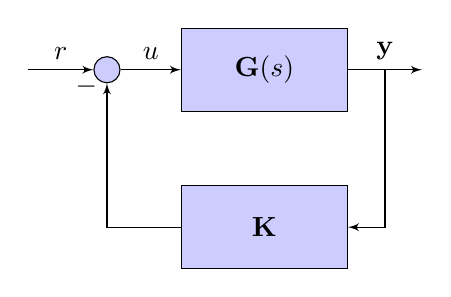
\begin{tikzpicture}[auto, node distance=2cm,>=latex']
    % We start by placing the blocks
    \node [input, name=input] {};
    \node [sum, right of=input] (sum) {};
    \node [block, right of=sum] (system) {$\mathbf{G}(s)$};
    % We draw an edge between the controller and system block to 
    % calculate the coordinate u. We need it to place the measurement block. 
    \node [output, right of=system] (output) {};
    \node [block, below of=system] (feedback) {$\mathbf{K}$};

    % Once the nodes are placed, connecting them is easy. 
    \draw [draw,->] (input) -- node {$r$} (sum);
    \draw [->] (sum) -- node {$u$} (system);
    \draw [->] (system) -- node [name=y] {$\mathbf{y}$}(output);
    \draw [->] (y) |- (feedback);
    \draw [->] (feedback) -| node[pos=0.99] {$-$} 
        node [near end] {} (sum);
  \end{tikzpicture}
  \caption{Block diagram of a feedback control system.}
  \label{fig:feedback_control_system}
\end{figure}

With feedback the new plant input is $u = w - \mathbf{Kx}$, where $\mathbf{K}$ is the control gain matrix.
This means that the closed loop transfer function is given by
\begin{equation}
  \mathbf{H}(s) = \frac{\mathbf{y}}{r} = \mathbf{C} (s\mathbf{I} - \mathbf{A} + \mathbf{KB}) ^{-1} \mathbf{B}
  \label{eq:closed_loop_tf}
\end{equation}

The poles of the closed loop transfer function are given by the roots of the characteristic polynomial
\begin{equation}
  \text{det} \left( s\mathbf{I} - \mathbf{A} + \mathbf{KB} \right) = 0
  \label{eq:det_poly}
\end{equation}

All poles must have a positive real part for the system to be stable.
The poles are the roots of a polynomial which means the Routh-Hurwitz criteria can be used.

\subsubsection{Crane Model}

For the crane model the equilibrium point is at $\theta = 0$ and $\dot{\theta} = 0$.
This means that equations \ref{eq:motion_1} and \ref{eq:motion_2} can be linearised about this point to give the equations:
\begin{align}
  \left( 1 + \frac{M}{m} + \frac{I}{ma^2} \right) \ddot{x} &= \frac{T}{ma} - \left(\frac{F}{m}\right)\text{sgn}(\dot{x}) + l \ddot{\theta} \label{eq:crane_motion_1} \\
  l \ddot{\theta} &= \ddot{x} - g\theta \label{eq:crane_motion_2}
\end{align}
These can be solved to give the state space model of the system.
\begin{align}
  \frac{d}{dt} \dot{x} &= \frac{mg}{l\left(M+\frac{I}{a^2}\right)} l\theta + u - f \\
  \frac{d}{dt} \dot{l\theta} &= -\frac{g}{l}l\theta + u - f
\end{align}
Where torque input $u$, and friction disturbance $f$, are defined as follows
\begin{equation}
  u = \frac{T}{a\left(M+\frac{I}{a^2}\right)} \quad \text{and} \quad f = \left(\frac{F}{M + \frac{I}{a^2}} \right) \text{sgn} (\dot{x})
  \label{eq:ss_system_inputs}
\end{equation}
The state space equations are in a form of simple harmonic motion with natural frequencies shown below,
\begin{align}
  \omega_1^2 &= \frac{g}{l} \\
  \omega_0^2 &= \omega_1^2\left(1 + \frac{m}{M+\frac{I}{a^2}} \right)
\end{align}
This gives the final state space model of the system as

\begin{equation}
  \frac{d}{dt} 
  \begin{bmatrix}
     x \\ \dot{x} \\ l\theta \\ \dot{l\theta} \end{bmatrix} = \begin{bmatrix} 
      0 & 1 & 0 & 0 \\ 0 & 0 & \omega_1^2 - \omega_0^2 & 0 \\ 0 & 0 & 0 & 1 \\ 0 & 0 & -\omega_0^2 & 0 \end{bmatrix} \begin{bmatrix} 
        x \\ \dot{x} \\ l\theta \\ \dot{l\theta} \end{bmatrix} + \begin{bmatrix} 
          0 \\ 1 \\ 0 \\ 1 \end{bmatrix} (u - f)
\end{equation}

\subsubsection{Inverted Pendulum Model}

For the inverted pendulum model the linearization is about the point $\theta = \pi$ and $\dot{\theta} = 0$.
The same quations of motion, \ref{eq:motion_1} and \ref{eq:motion_2}, are substituted with $\theta = \pi - \phi$.
\begin{align}
  \left( 1 + \frac{M}{m} + \frac{I}{ma^2} \right) \ddot{x} &= \frac{T}{ma} - \frac{F}{m}\text{sgn}(\dot{x}) - l\sin\phi . \ddot{\phi} - l\cos\phi . \dot{\phi}^2 \\
   - l \ddot{\phi} &= \sin\phi \ddot{x} - g\cos\phi
\end{align}
The new states become $\mathbf{x} = \left[ x \quad \dot{x} \quad l\phi \quad l\dot{\phi} \right]^T$

linearising equations \ref{eq:motion_1} and \ref{eq:motion_2} yield the following:
\begin{align}
  \left( 1 + \frac{M}{m} + \frac{I}{ma^2} \right) \ddot{x} &= \frac{T}{ma} - \left(\frac{F}{m} \right)\text{sgn}(\dot{x}) + l \ddot{\phi} \label{eq:invp_motion_1} \\
  l \ddot{\phi} &= \ddot{x} + g\phi \label{eq:invp_motion_2}
\end{align}

The states can be substituted and solved for the state space model in terms of the same input $u$ and disturbance $f$ as the crane model defined in equation \ref{eq:ss_system_inputs}.

\begin{equation}
  \frac{d}{dt} 
  \begin{bmatrix}
     x \\ \dot{x} \\ l\phi \\ \dot{l\phi} \end{bmatrix} = \begin{bmatrix} 
      0 & 1 & 0 & 0 \\ 0 & 0 & \omega_0^2 - \omega_1^2 & 0 \\ 0 & 0 & 0 & 1 \\ 0 & 0 & \omega_0^2 & 0 \end{bmatrix} \begin{bmatrix} 
        x \\ \dot{x} \\ l\phi \\ \dot{l\phi} \end{bmatrix} + \begin{bmatrix} 
          0 \\ 1 \\ 0 \\ 1 \end{bmatrix} (u - f)
\end{equation}

\subsection{Closed loop control}


\subsubsection{Crane}

From equation \ref{eq:det_poly} the closed loop characteristic polynomial of the crane model is given by
\begin{equation}
  s^{4} + \left(k_{2} + k_{4}\right) s^{3} + \left(k_{1} + k_{3} + \omega_{0}^{2}\right) s^{2} + k_{2} \omega_{1}^{2} s + k_{1} \omega_{1}^{2}
  \label{eq:crane_poly}
\end{equation}
Application of the Ruth Hurwitz criteria gives the following conditions for stability
\begin{align}
  k_{2} + k_{4} &> 0 \\
  k_{1} + k_{3} + \omega_{0}^{2} &> 0 \\
  k_{2} \omega_{1}^{2} &> 0 \\
  \left(k_{3} + \omega_{0}^{2} - \omega_{1}^{2}\right) k_{2}^{2} + \left(- k_{1} k_{4} + k_{3} k_{4} + k_{4} \omega_{0}^{2}\right) k_{2} -  k_{1} k_{4}^{2} &> 0
\end{align}

At the point of marginal stability $s = \pm j\hat{\omega}$.
From substituting this into the characteristic polynomial \ref{eq:crane_poly} and considering both real and imaginary coefficients the following equations are found

\begin{align}
    - \hat{\omega}^{3} \left(k_{2} + k_{4}\right) + k_{2} \omega_{1}^{2} \hat{\omega}  &= 0 \\
    \hat{\omega}^{4} - \left(k_{1} + k_{3} + \omega_{0}^{2}\right)\hat{\omega}^{2} + k_{1} \omega_{1}^{2} &= 0
\end{align}

The first equation can be solved for the frequency $\hat{\omega}$ and substituted into the second equation to give:
\begin{align}
  \begin{gathered}
    \hat{\omega} = \sqrt{\frac{k_2}{k_2 + k_4}} \omega_1 \label{eq:marginal_stability_frequency}\\
    \frac{\omega_1^2}{(k_2+k_4)^2} \left( \left(k_{3} + \omega_{0}^{2} - \omega_{1}^{2}\right) k_{2}^{2} + \left(- k_{1} k_{4} + k_{3} k_{4} + k_{4} \omega_{0}^{2}\right) k_{2} -  k_{1} k_{4}^{2} \right) = 0
  \end{gathered}
\end{align}
The second result shows that the last condition for stability becomes an equality at the point of marginal stability.
The value of $k_2$ can be found by solving this equation and the solution is shown below.

\begin{equation}
  k_2 = \frac{k_{4} \left(k_{1} - k_{3} - \omega_{0}^{2} \pm \sqrt{k_{1}^{2} + 2 k_{1} k_{3} + 2 k_{1} \omega_{0}^{2} - 4 k_{1} \omega_{1}^{2} + k_{3}^{2} + 2 k_{3} \omega_{0}^{2} + \omega_{0}^{4}}\right)}{2 \left(k_{3} + \omega_{0}^{2} - \omega_{1}^{2}\right)}
  \label{eq:predicted_crane_k2}
\end{equation}
When this solution is substituted back into the characteristic polynomial

\subsubsection{Inverted Pendulum}

From equation \ref{eq:det_poly} the closed loop characteristic polynomial of the inverted pendulum model is given by

\begin{equation}
  s^{4} + \left(k_{2} + k_{4}\right) s^{3} + \left(k_{1} + k_{3} - \omega_{0}^{2}\right) s^{2} -  k_{2} \omega_{1}^{2} s -  k_{1} \omega_{1}^{2}
  \label{eq:pendulum_poly}
\end{equation}

Application of the Ruth Hurwitz criteria gives the following conditions for stability
\begin{align}
  k_{2} + k_{4} &> 0 \\
  k_{1} + k_{3} - \omega_{0}^{2} &> 0 \\
  - k_{2} \omega_{1}^{2} &> 0 \\
  \left(- k_{3} + \omega_{0}^{2} - \omega_{1}^{2}\right) k_{2}^{2} + \left(k_{1} - k_{3} + \omega_{0}^{2}\right) k_{4} k_{2} + k_{1} k_{4}^{2} &> 0
\end{align}

At the point of marginal stability $s = j\hat{\omega}$.
From substituting this into the characteristic polynomial \ref{eq:pendulum_poly} and considering both real and imaginary coefficients the following equations are found

\begin{align}
  - \hat{\omega}^{3} \left(k_{2} + k_{4}\right) - \hat{\omega} k_{2} \omega_{1}^{2} &= 0\\
  \hat{\omega}^{4} - \hat{\omega}^{2} \left(k_{1} + k_{3} - \omega_{0}^{2}\right) - k_{1} \omega_{1}^{2} &= 0
\end{align}
This gives the same frequency as the crane model \ref{eq:marginal_stability_frequency}. This is substituted back into the second equation to give:
\begin{equation}
  \frac{\omega_1^2}{(k_2 + k_4)^2} \left( \left(- k_{3} + \omega_{0}^{2} - \omega_{1}^{2}\right) k_{2}^{2} + \left(k_{1} - k_{3} + \omega_{0}^{2}\right) k_{4} k_{2} + k_{1} k_{4}^{2} \right) = 0
\end{equation}
This is again the same as the last condition for stability becoming an equality at the point of marginal stability.
The value of $k_2$ at the point of marginal stability is found by solving this equation and the solution is shown below.

\begin{equation}
  k_2 = \frac{k_{4} \left(k_{1} - k_{3} - \omega_{0}^{2} - \sqrt{k_{1}^{2} + 2 k_{1} k_{3} + 2 k_{1} \omega_{0}^{2} - 4 k_{1} \omega_{1}^{2} + k_{3}^{2} + 2 k_{3} \omega_{0}^{2} + \omega_{0}^{4}}\right)}{2 \left(k_{3} + \omega_{0}^{2} - \omega_{1}^{2}\right)}
\end{equation}

\subsubsection{Eigenvalue Sensitivity}

The roots of a polynomial can be very sensitive to coefficients, particularly when roots are nearly repeated.
This is shown by considering the polynomial
\begin{equation}
  d(s) = (s+k)^4 + \epsilon k^4
\end{equation}
For $\epsilon = 0$ the polynomial has a fourth order repeated root at $s = -k$.
However, even for small $\epsilon$ the roots of the polynomial can vary significantly. This is shown below in figure \ref{fig:pole_sensitivity}.

\begin{figure}[H]
  \centering
  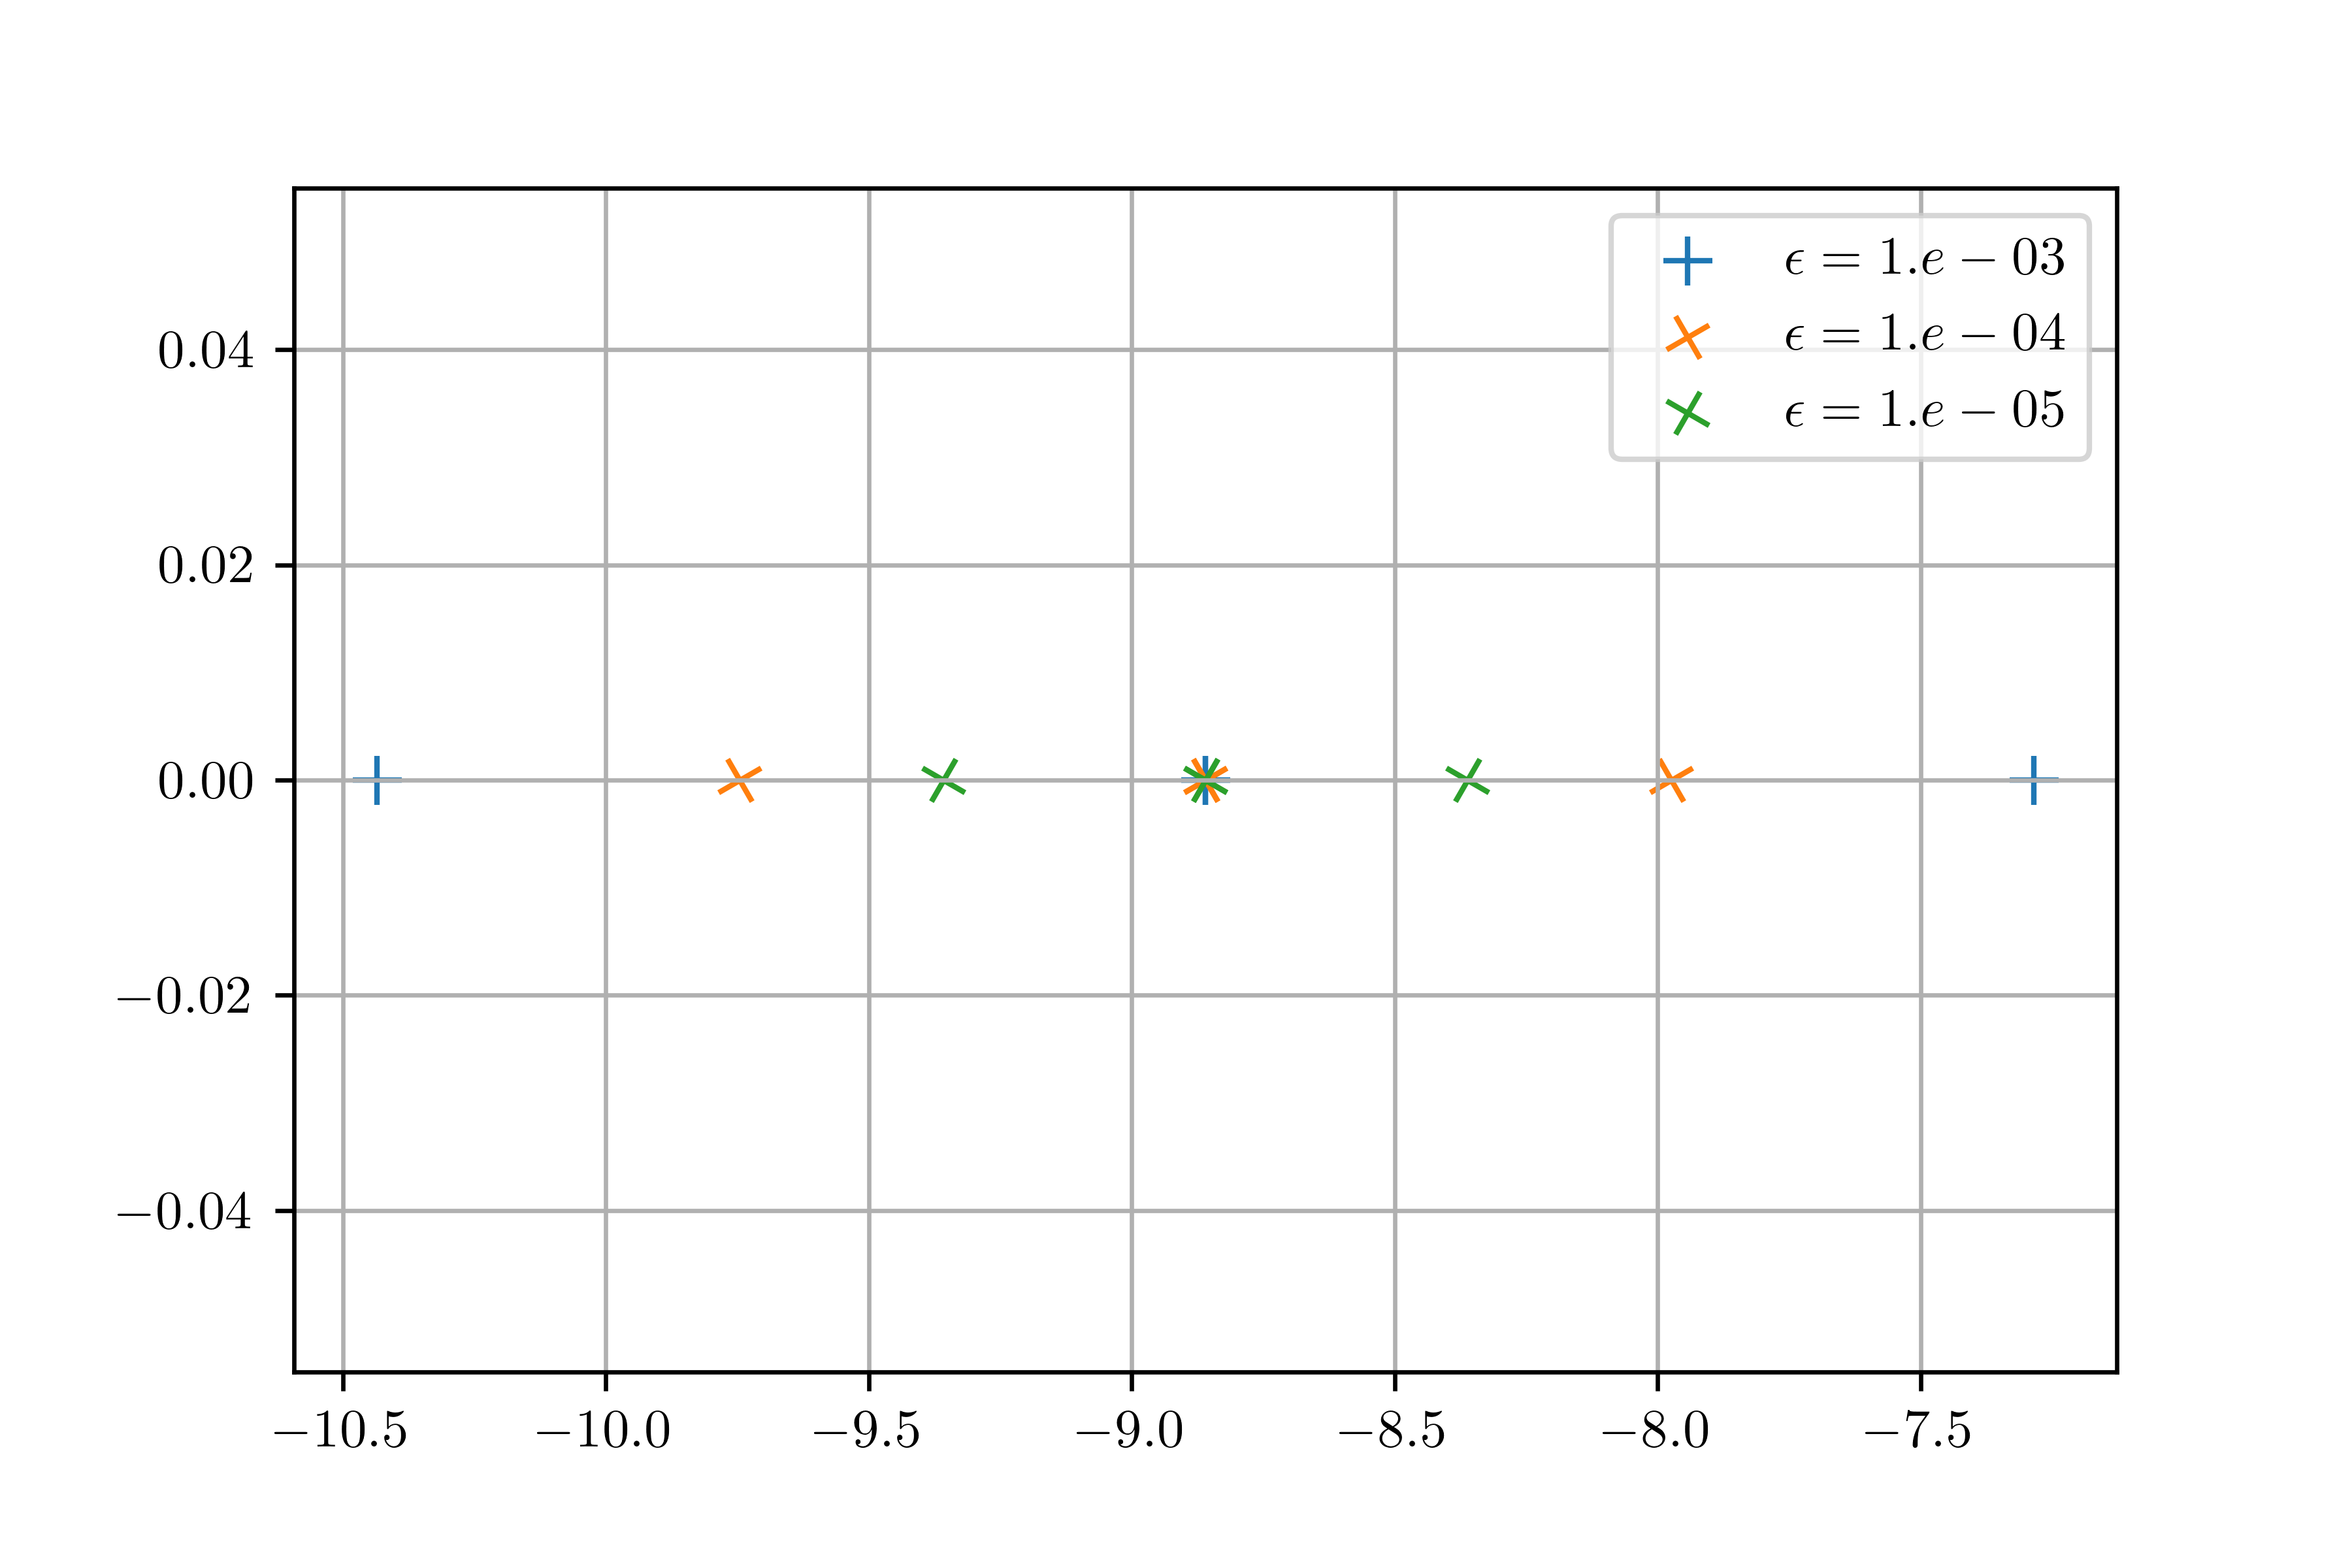
\includegraphics[width=0.6\textwidth]{figures/pole_sensitivity.png}
  \caption{Variation of the roots of a polynomial for small perturbations in the coefficient, $\epsilon$.}
  \label{fig:pole_sensitivity}
\end{figure}

\subsection{Nonlinear Friction term}
So far we have only considered linear theory, however the sign function in the friction term $f$ cannot be linearised.
The describing function method can be used to find the frequency-response function for
the nonlinear friction.
The following analysis will be on single output systems, however the method can be extended to each output.

\begin{figure}[H]
  \centering
  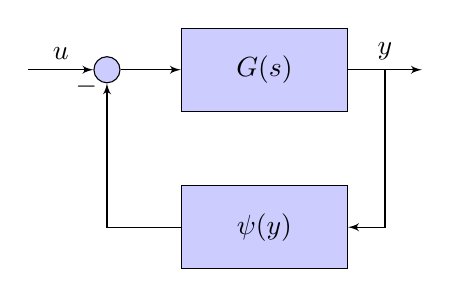
\begin{tikzpicture}[auto, node distance=2cm,>=latex']
    % We start by placing the blocks
    \node [input, name=input] {};
    \node [sum, right of=input] (sum) {};
    \node [block, right of=sum] (system) {$G(s)$};
    % We draw an edge between the controller and system block to 
    % calculate the coordinate u. We need it to place the measurement block. 
    \node [output, right of=system] (output) {};
    \node [block, below of=system] (feedback) {$\psi(y)$};

    % Once the nodes are placed, connecting them is easy. 
    \draw [draw,->] (input) -- node {$u$} (sum);
    \draw [->] (sum) -- node {} (system);
    \draw [->] (system) -- node [name=y] {$y$}(output);
    \draw [->] (y) |- (feedback);
    \draw [->] (feedback) -| node[pos=0.99] {$-$} 
        node [near end] {} (sum);
  \end{tikzpicture}
  \caption{Nonlinearity $\psi(y)$ }
  \label{fig:nonlinear_block_diagram}
\end{figure}

From the \textit{harmonic balance equation} \cite{non_linear_systems}, $\Psi(E)G(j\omega) + 1 = 0$.
The function $\Psi(E)$ "describes" the nonlinearity $\psi$ for a harmonic input of amplitude $E$ which is defined below.
This is also in the form of an additional feedback gain for $k_2$.

\begin{equation}
  \Psi(E) = \frac{2}{\pi E} \int_0^{\pi} \psi(E\sin\theta)\sin\theta d\theta
\end{equation}

However, its important to note that this method neglects higher order harmonics, assuming that the transfer function $H(j\omega)$ have sharp low pass filtering characteristics.
In the case of the sign function for friction, the nonlinearity is given by 
\begin{equation}
  \psi(\mathbf{y}) = \left(\frac{F}{M + \frac{I}{a^2}} \right) \text{sgn}(\dot{x})
\end{equation}

This gives the additional gain due to the nonlinearity as
\begin{align}
  \Psi(E) &= \frac{2}{\pi E} \left(\frac{F}{M + \frac{I}{a^2}} \right) \int_0^{\pi} \text{sgn}(E\sin\theta)\sin\theta d\theta \\
          &= \frac{4}{\pi E} \frac{F}{M + I/{a^2}}
\end{align}


\subsection{Linear Quadratic Regulator}

The cost function associated with optimal control

\begin{equation}
  J = \int_0^\infty \left( \mathbf{x}^T \mathbf{Q} \mathbf{x} + \mathbf{u}^T \mathbf{R} \mathbf{u} \right) dt
\end{equation}

Where the matricies $\mathbf{Q}$ and $\mathbf{R}$ are the diagonal state and control weighting matricies respectively.
They are chosen using Bryson's rule, a heuristic method for choosing the matricies shown below 

\begin{equation}
  \mathbf{Q}_{ii} = \frac{1}{\text{max}(\mathbf{x}_i)^2} \quad \mathbf{R} = \frac{1}{\text{max}(u)^2}
\end{equation}

Where max is an approximation for the maximum desired value of the state or control input.
From this the response can be tuned to 

\subsubsection{Optimal Performance Evaluation}

The real world performance of the LQR determined system gains can be observed by measuring the input power and the response.

\section{Method}

\subsection{Apparatus}

Two digital optical encoders were used to measure the position of the crane and the carriage.
These were numerically differentiated on microcontrollers to give the velocity of the crane and carriage.
These were then all converted to an analog signal and amplified by entered gains and selected controller signs.
The signals are summed and drive the current to the 3 phase brushless motor. 
The analog demand and state signals were converted digitally at a rate of 400 Hz to a computer for data logging. 

\begin{figure}[H]
  \centering
  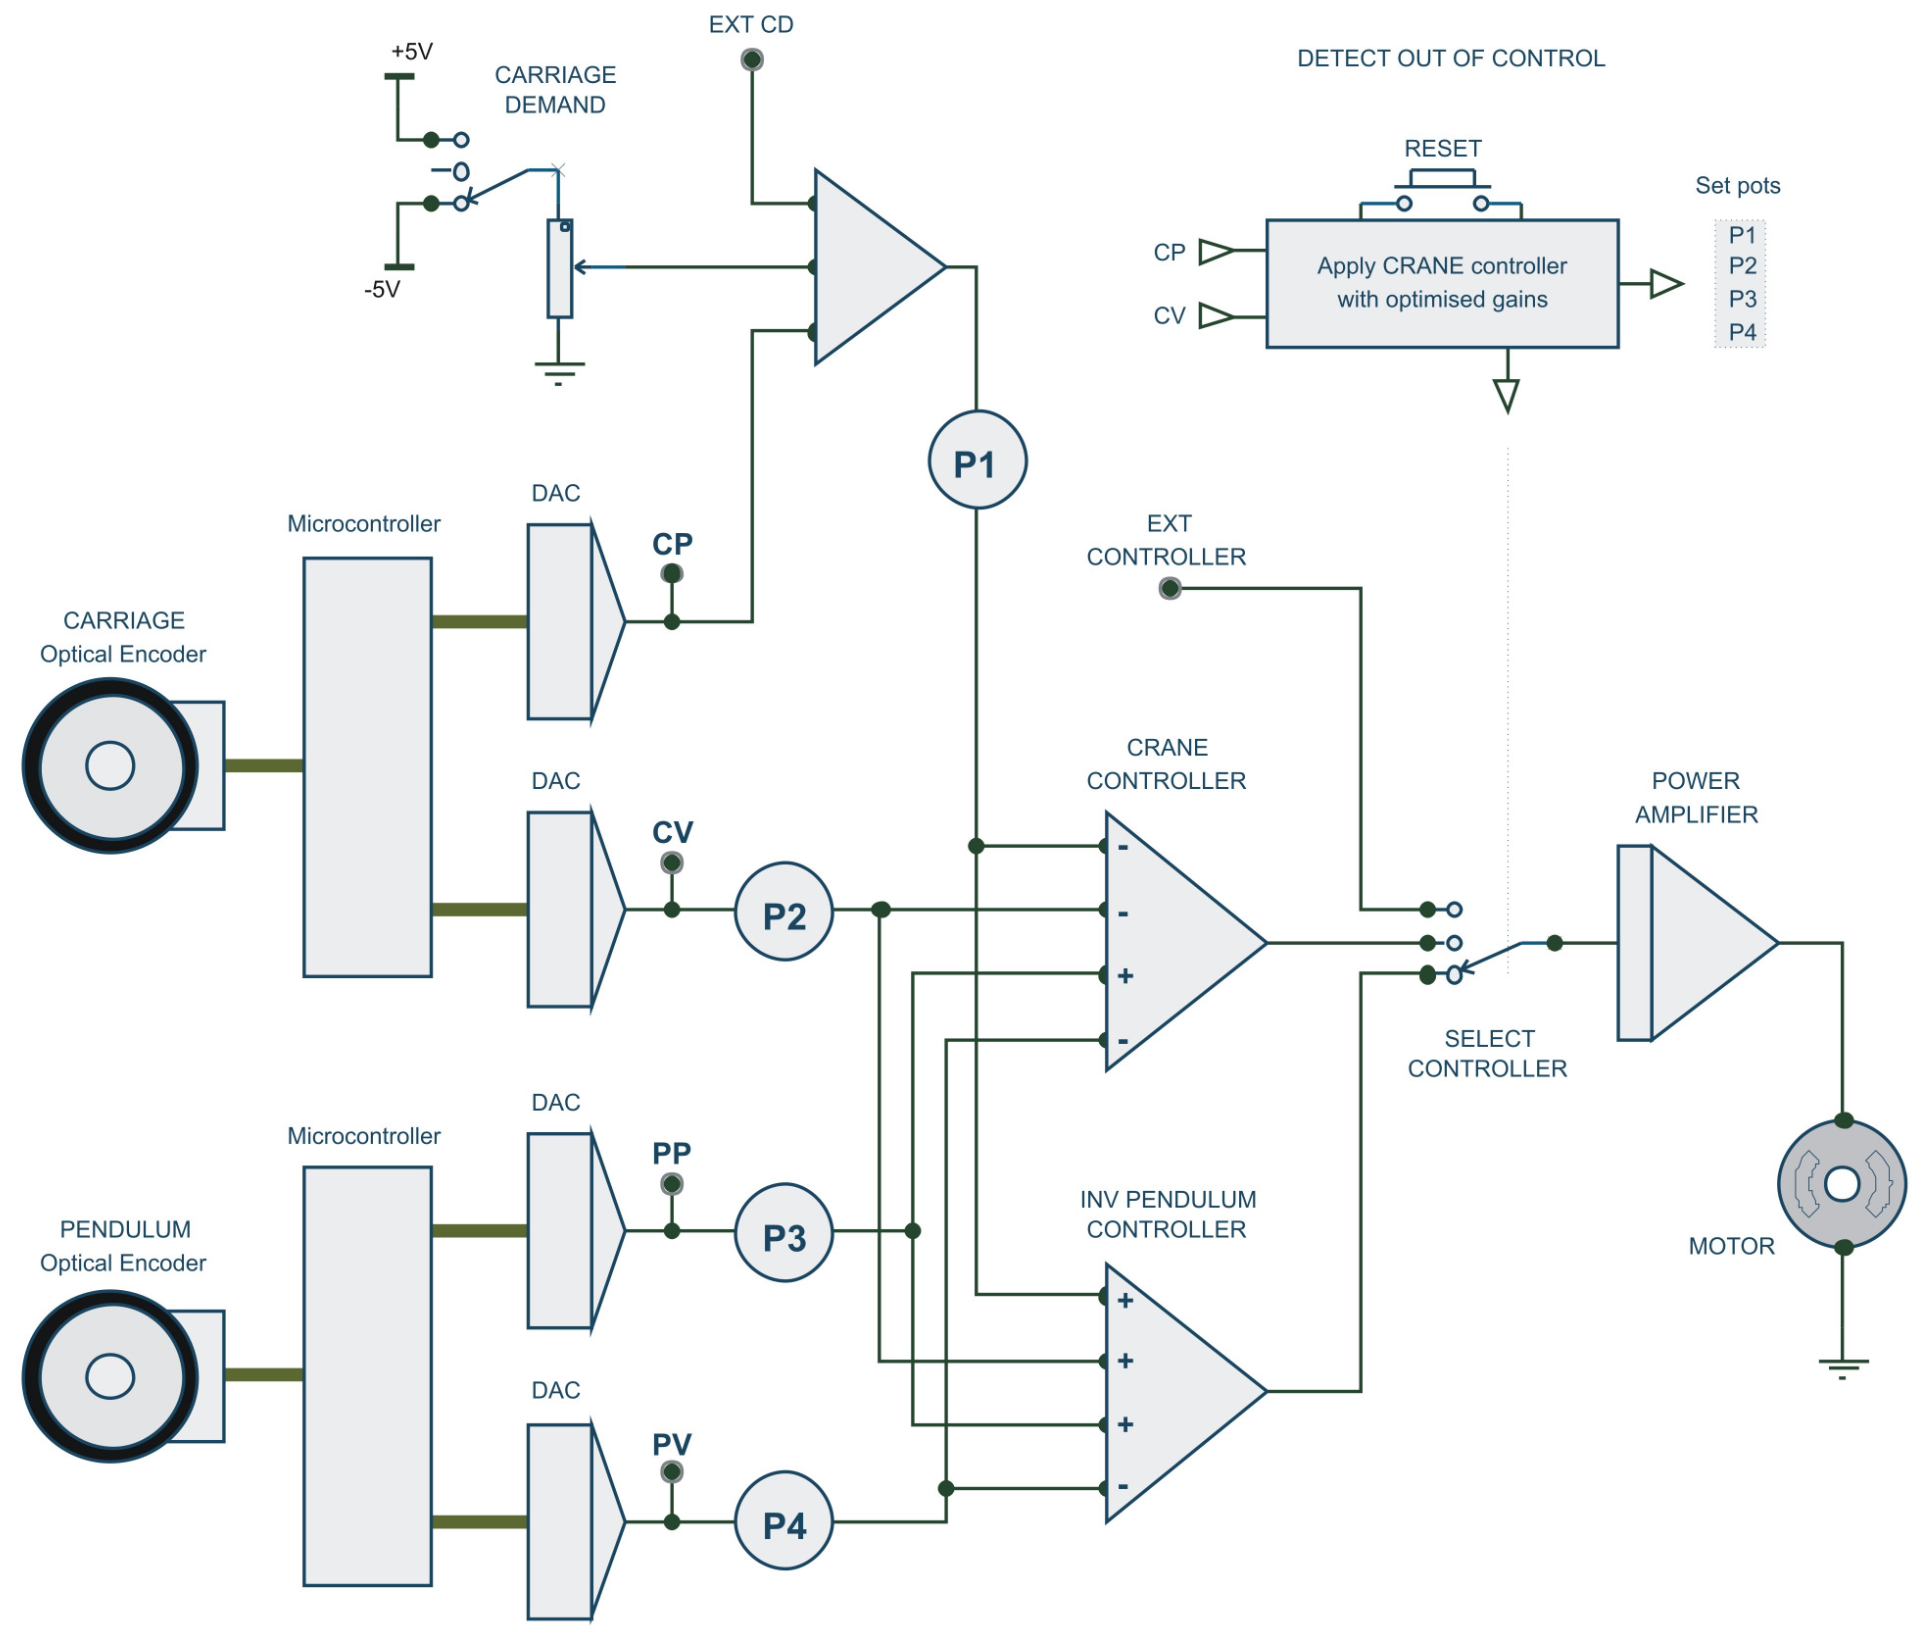
\includegraphics[width=0.6\textwidth]{figures/electrical_layout.png}
  \caption{Circuit block diagram for the electrical layout of the system.}
  \label{fig:electrical_layout}
\end{figure}

\subsection{Procedure}


%\iffalse
%-----------------------------------------------------------------------------------------
\section{Results and Discussion}
%-----------------------------------------------------------------------------------------

\subsection{Crane}

\subsubsection{Friction Measurement}

\subsubsection{Carriage Controller}

\subsubsection{Empirical synthesis of $p_3$ and $p_4$ controller}

\begin{figure}[H]
  \centering
  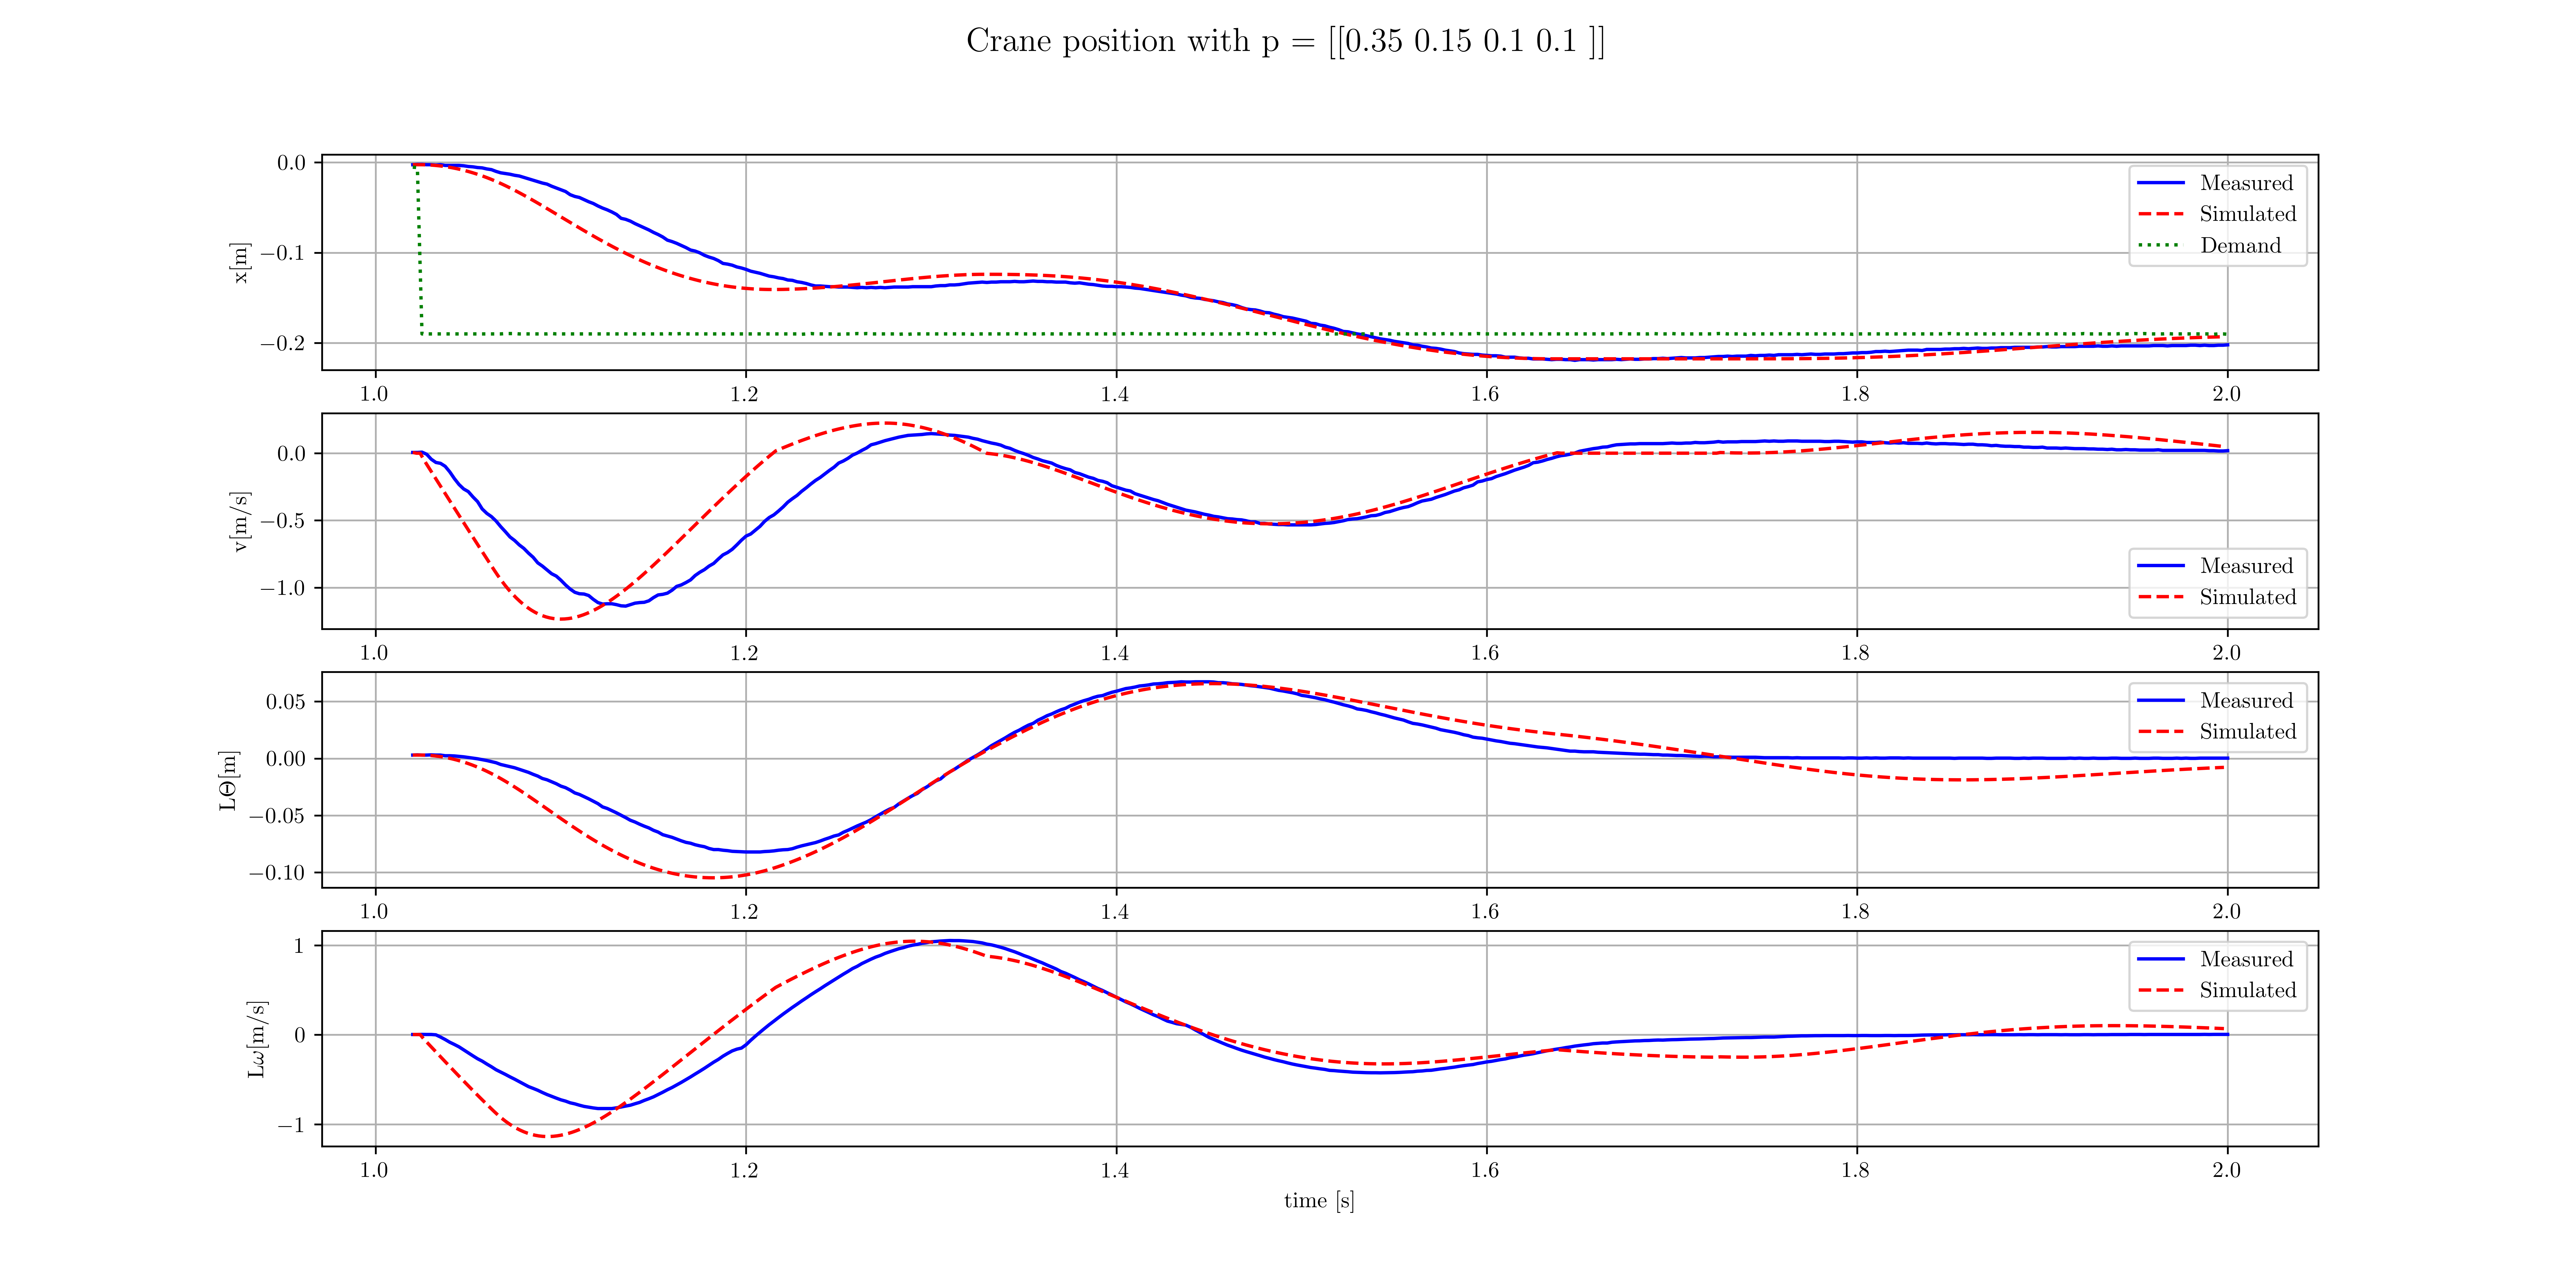
\includegraphics[width=0.99\textwidth]{figures/3.3.png}
  \caption{}
  \label{fig:exp3.3}
\end{figure}

From figure \ref{fig:exp3.3} the oscillatory response of the carriage velocity was measured to give a period of 0.36s giving a frequency of 17.45 rad/s.
The response also shows moderate damping where the amplitude of carriage velocity halved over about 1 period, giving a damping ratio of $\zeta \approx 0.11$.

From the closed loop gain setpoints the pole locations are calculated as: \\
$[-3.89861823 \pm 18.69316043j, -2.16928301 \pm 6.46486529j]$
These indicate a highly damped system with frequency responses of 18.7 and 6.5 rad/s and corresponding damping ratios of 0.208 and 0.336.

The frequency is consistent with the calculated pole locations. The measured damping ratio is slightly lower than expected, 
which is likely due to high uncertainty in the periods over which the amplitude halved, and the rule of thumb method used requiring small damping ratios to be valid.

There is a small discrepency between the simulated and observed responses. This is due to uncertainty in system parameters rather than numerical error in the verlet integrator method.
Uncertainty in the system parameters include the sensor constants, amplifier gains, friction coefficients, mass and moments of inertia of the system.

As expected, the 

\subsubsection{Pole Placement}

\begin{figure}[H]
  \centering
  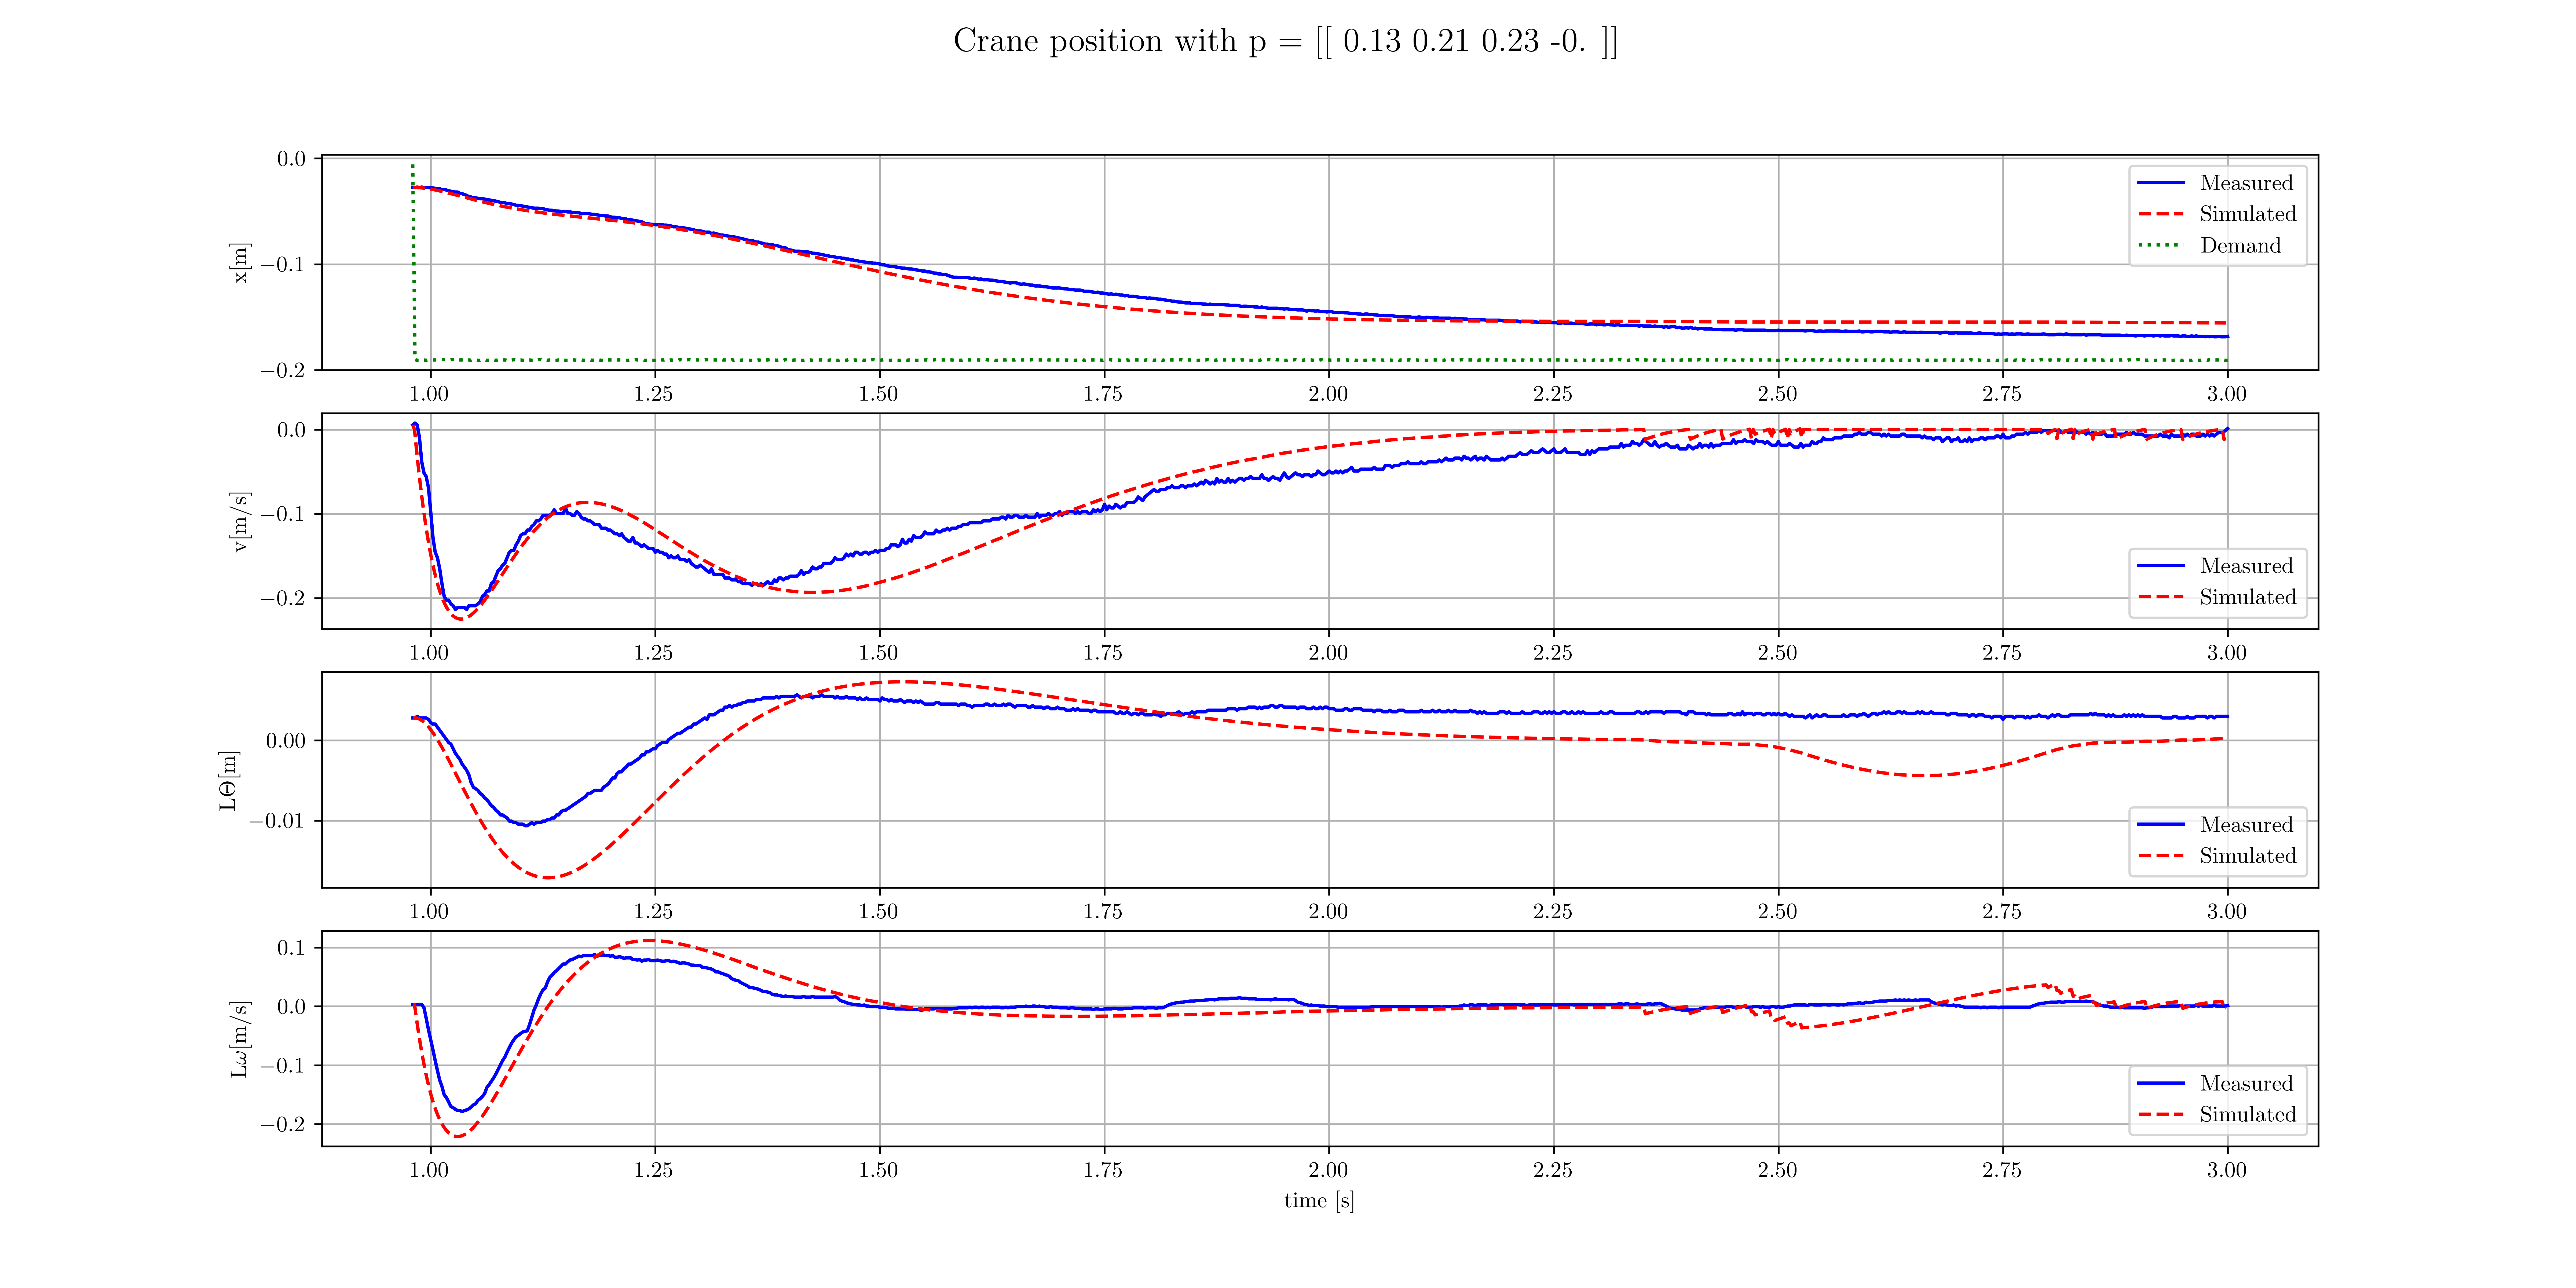
\includegraphics[width=0.99\textwidth]{figures/3.4a.png}
  \caption{All poles at $-\omega_1 = -\sqrt{78.5}$}
  \label{fig:exp3.4a}
\end{figure}

% After carefully calculating the poles using $k_1 = \omega_1^2$, $k_2 = 4\omega_1$, $k_3 = 5\omega_1^2 - \omega_0^2$ and finally $k_4 = 0$
The gains were calculated from equating expanded coefficients of $(s - \omega_1)^4$ with the characteristic polynomial \ref{eq:crane_poly}.
These were found to be $[ 0.13,  0.21,  0.23, 0.00 ]$, rounded to 2 decimal places which was the maximum precision of the potentiometers.

The calculated poles from these rounded values were found to be $[-12.45360996 \pm 6.46216554j, -4.89083448 \pm 2.84116008j]$.
This shows that the poles are not consistent with the target pole position.
Figure \ref{fig:pole_sensitivity} demonstrates the high sensitivity of the pole locations to small variations of coefficients in the characteristic polynomial.
This explains why the position of the 2 decimal place rounded gains are so far from the target pole positions.

\begin{figure}[H]
  \centering
  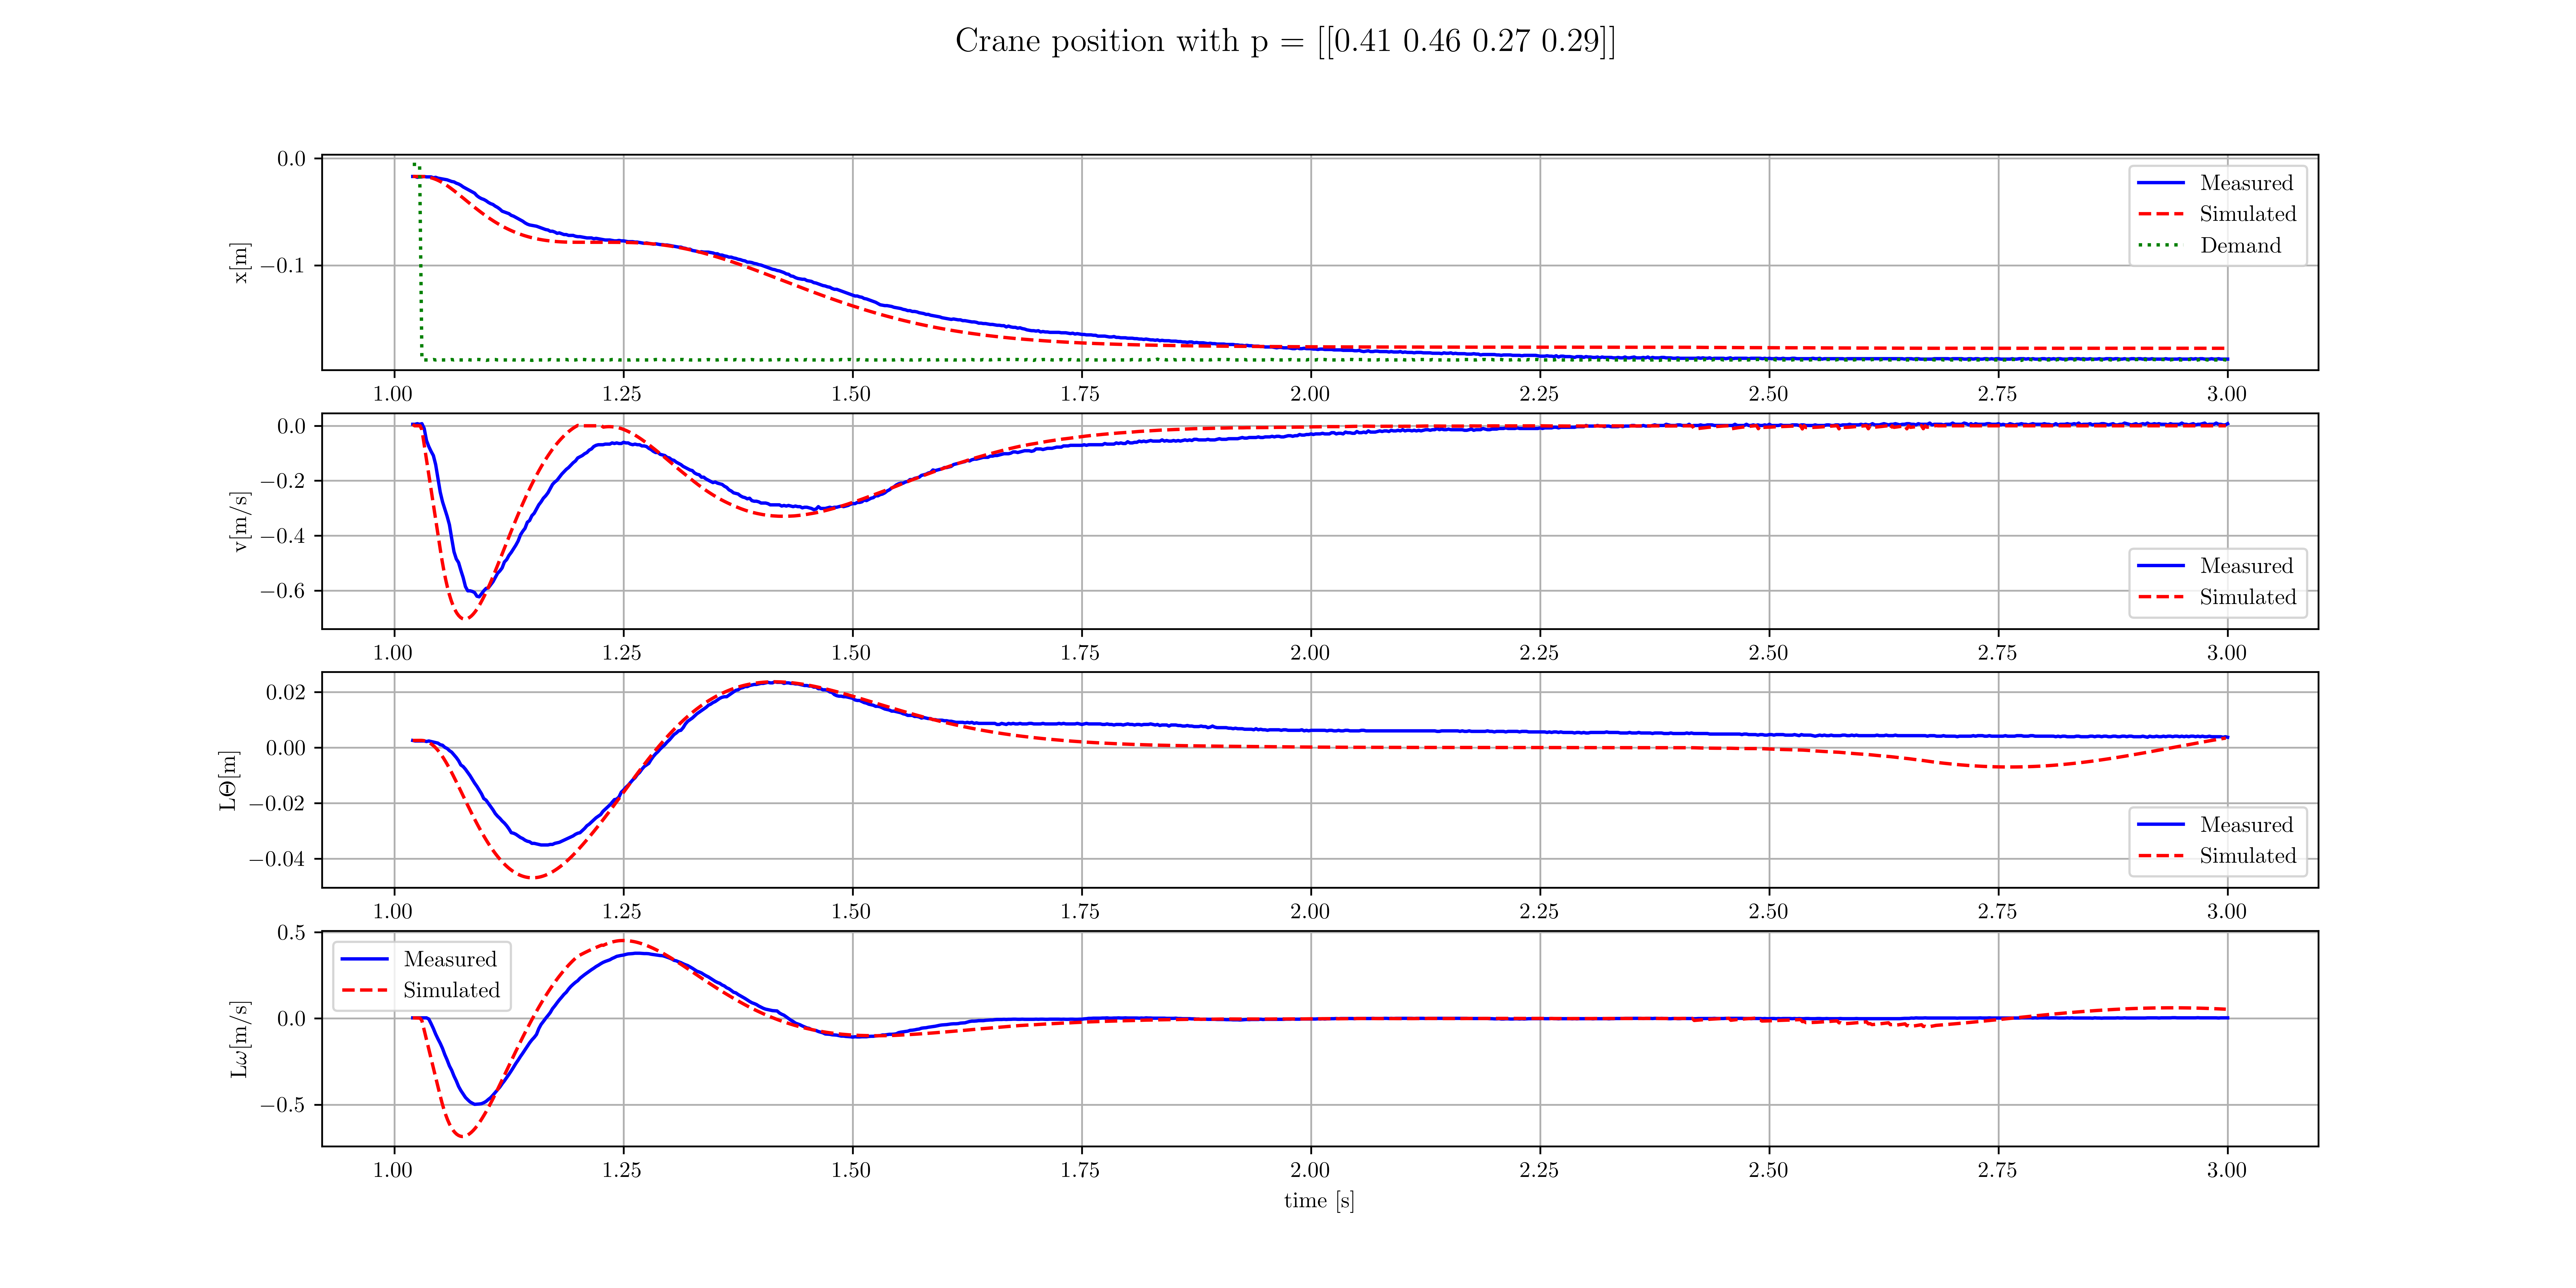
\includegraphics[width=0.99\textwidth]{figures/3.4b.png}
  \caption{Poles at $-\alpha, -\beta, -\omega \pm j\omega$ where $\alpha = \beta = \omega = 10$}
  \label{fig:exp3.4b}
\end{figure}

Figure \ref{fig:exp3.4b} shows the response for gains calculated at chosen pole locations, $-\alpha, -\beta, -\omega \pm j\omega$.
The values were chosen as $\alpha = 10; \beta= 10; \omega = 10$ for which the gain values were calculated by expanding the polynomial from the roots and equating
coefficients with the characteristic polynomial \ref{eq:crane_poly}.
These were found to be $[0.41284404 \quad 0.46282964 \quad 0.27212883 \quad 0.28834576]$

The poles at the rounded gain values are found to be $[-10.34437835 \pm 10.61053723j, \quad -9.31735005 \pm 1.90749139j]$ 
which is quite close to the design point of a repeated pole at $-10$, and poles at -$10\pm 10j$

The response shows some oscillation components, but the system is highly damped and the frequency response is difficult to measure.
This makes it difficult to compare the observed response with the pole locations.

The simulated response shows a lower frequency of about ???

\subsubsection{Variation of $p_2$}

\begin{figure}[H]
  \centering
  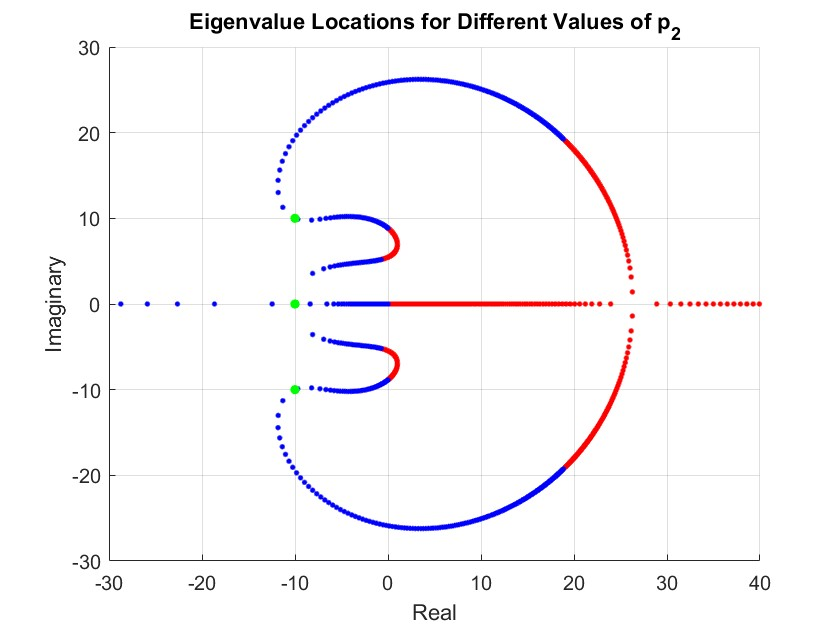
\includegraphics[width=0.7\textwidth]{figures/3.5roots.jpg}
  \caption{Crane root locus for varying $k_2$ only}
  \label{fig:roots3.5}
\end{figure}

\begin{figure}[H]
  \centering
  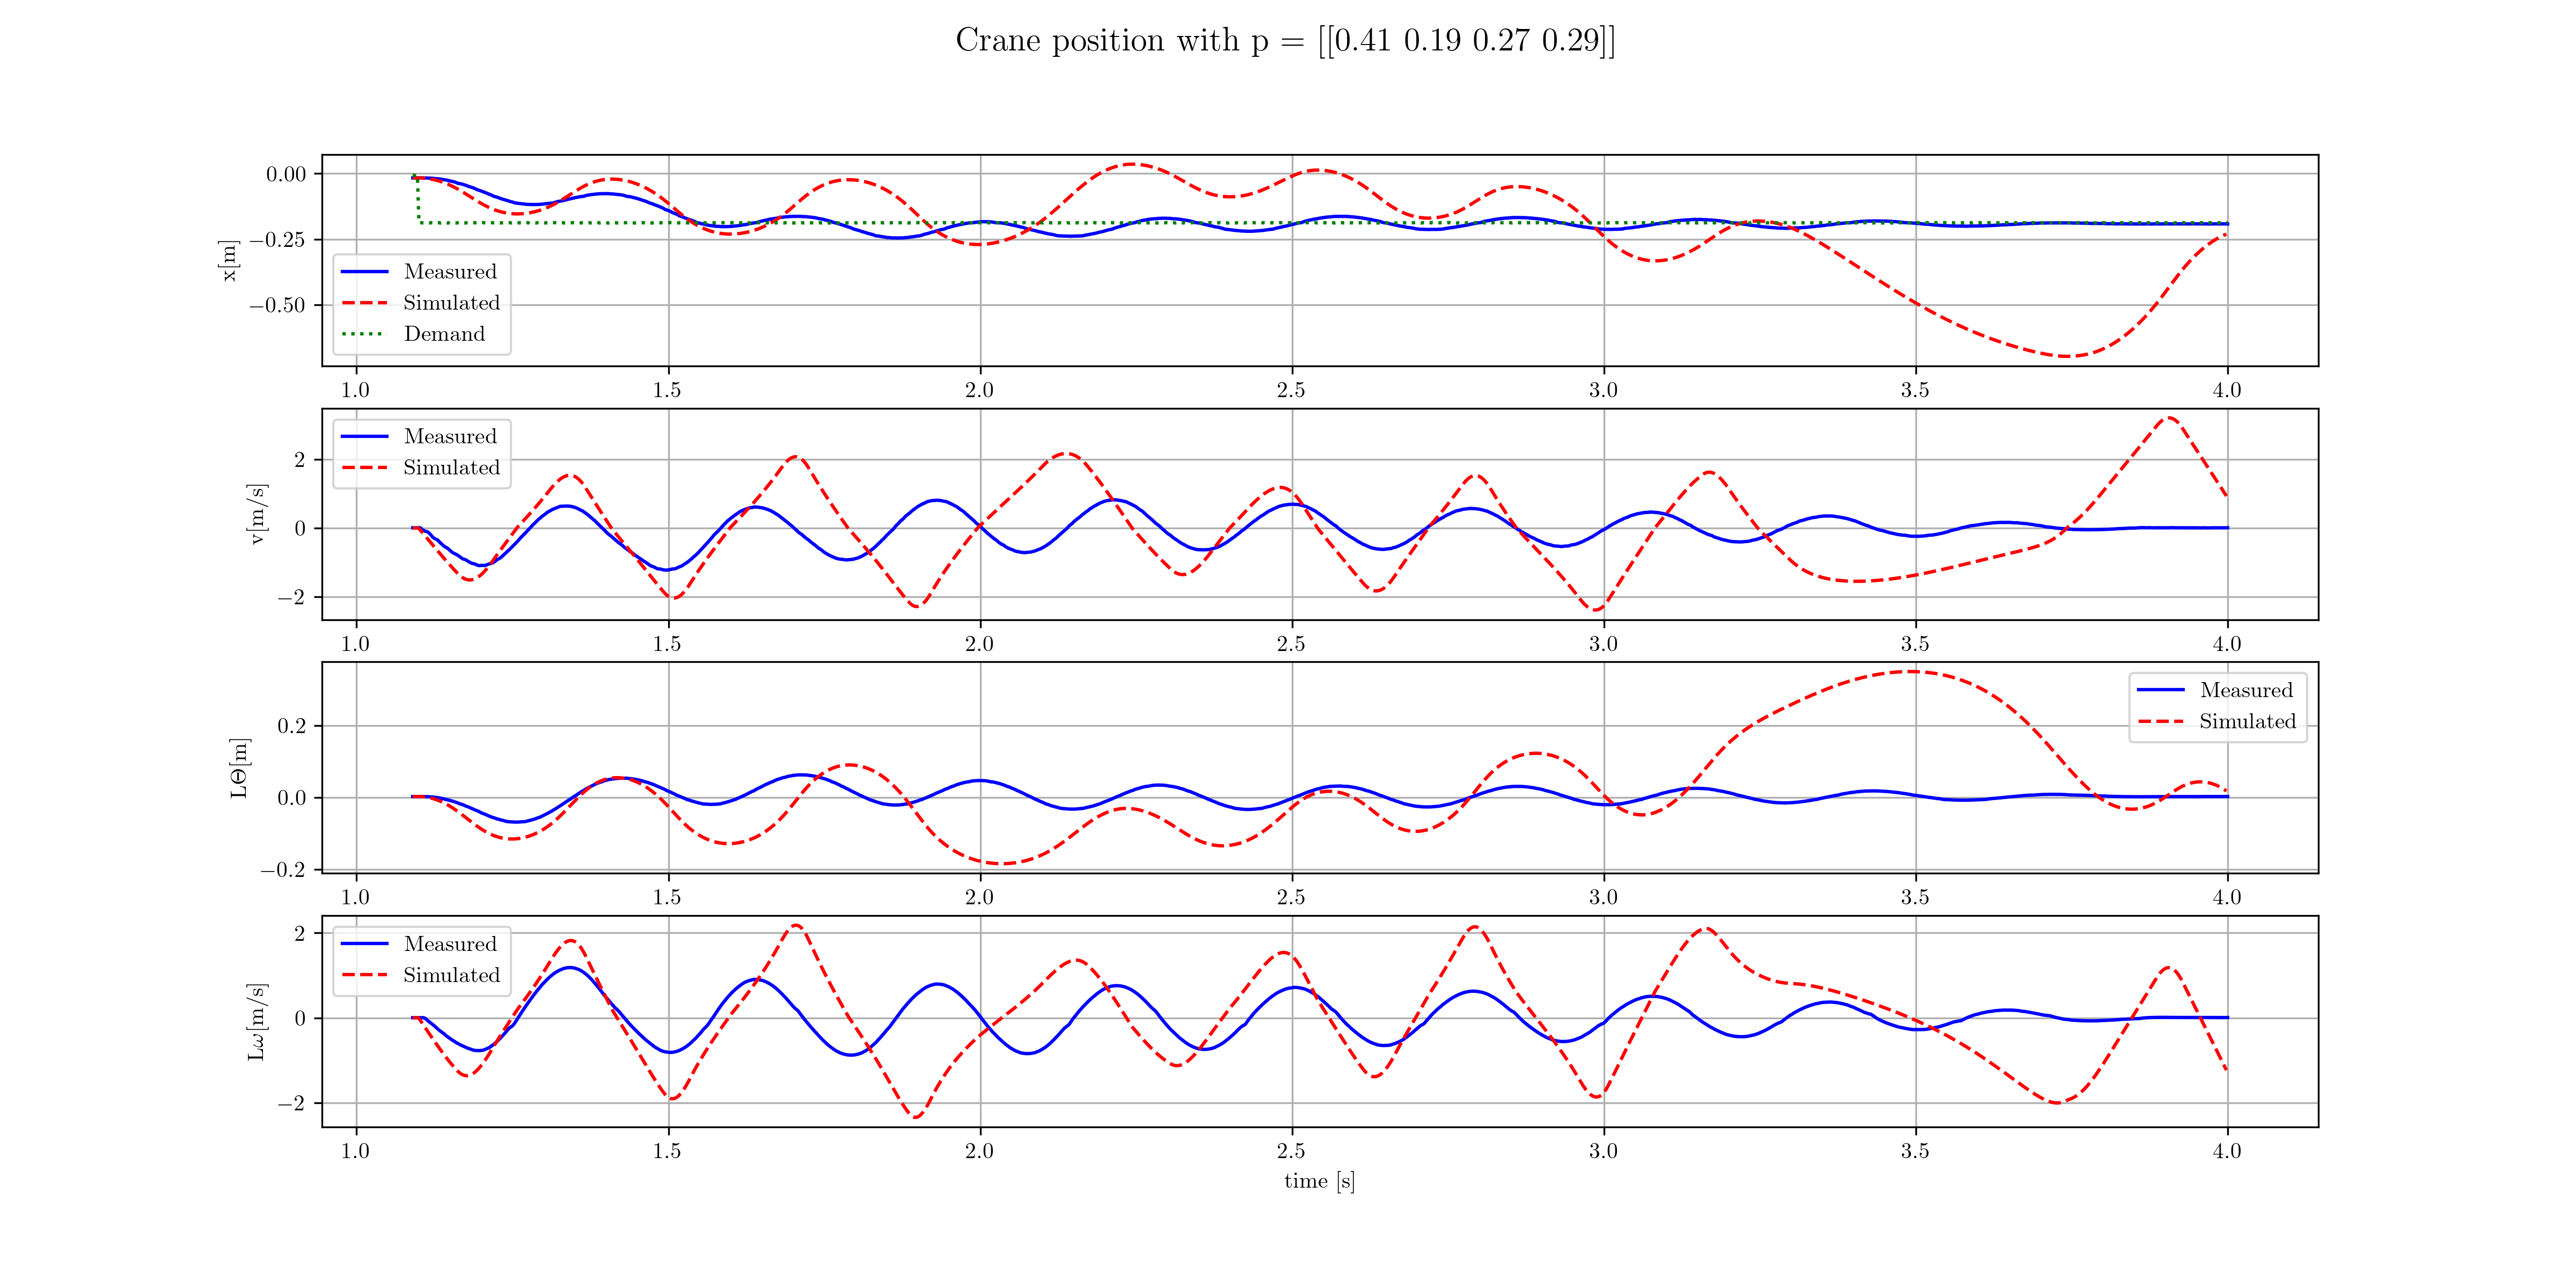
\includegraphics[width=0.99\textwidth]{figures/3.5.png}
  \caption{Limit of stability}
  \label{fig:exp3.5}
\end{figure}

Figure \ref{fig:exp3.5} shows the response for the smallest $k_2$ where instability starts to occur.
The value of $p_2$ reduced from 0.46 to 0.19 which corresponds to $k_2 = 31.35$
The measured frequency was $21.67$ rad/s and the amplitude of velocity of the carriage dropped to half of the maximum value after 4 cycles, giving the damping ratio as $\zeta \approx 0.03$

From equation \ref{eq:predicted_crane_k2} the predicted gain at the onset of instability $k_2 = 41.43$ and frequency $\hat{\omega} = 25.76$ Rad/s
Additionally, the theoretical closed loop pole locations were found as \\ 
$[ 4.57476482 \pm 26.11156105j , \quad -1.93649322 \pm 4.95114934j]$
The first two poles that lie to the right of the imaginary axis suggests that the system should be unstable for this value of $p_2 = 0.19$.

Both of these indicate that the lower bound gain $k_2$ at the onset of unstability is smaller than expected. This means that the system is more stable than predicted by the linear model.

%%% This is becuase of the additional gain from friction in the real system.
From theory covered in A6 of the appendix, the onset of instability is related to friction in the limit cycles which is not considered in linear theory.
For small oscillations the real system has a large additional damping term from friction, which is why the linear model predicts instability to occur at a higher gain than observed.
At a gain of $p_2 = 0.18$ oscillations occur at larger amplitudes and so according to A6 the additional damping from friction is smaller which causes the system to become unstable.

%---------------------------------------------------------------------------------------------------------------------
\subsection{Inverted Pendulum}
%---------------------------------------------------------------------------------------------------------------------

\subsubsection{No Carriage Feedback}

% No Carriage feedback
%% EXPLAIN BEHAVIOUR
The pendulum position drifts away from the zero position with increasing carriage velocity showing unstability.
A first test showed that even a very small pendulum angle caused an initial motion of the carriage.
On another test, the pendulum was carefully left at an initial angle of zero, where it was stationary.
A very small force displaced the pendulum and the carriage accelerated away from the zero position. 

This unstability is predicted by the poles of the system, where there is a repeated pole at 0


\subsubsection{Pole Placement}
% 4.3 pole placement at -omega1
\begin{figure}[H]
  \centering
  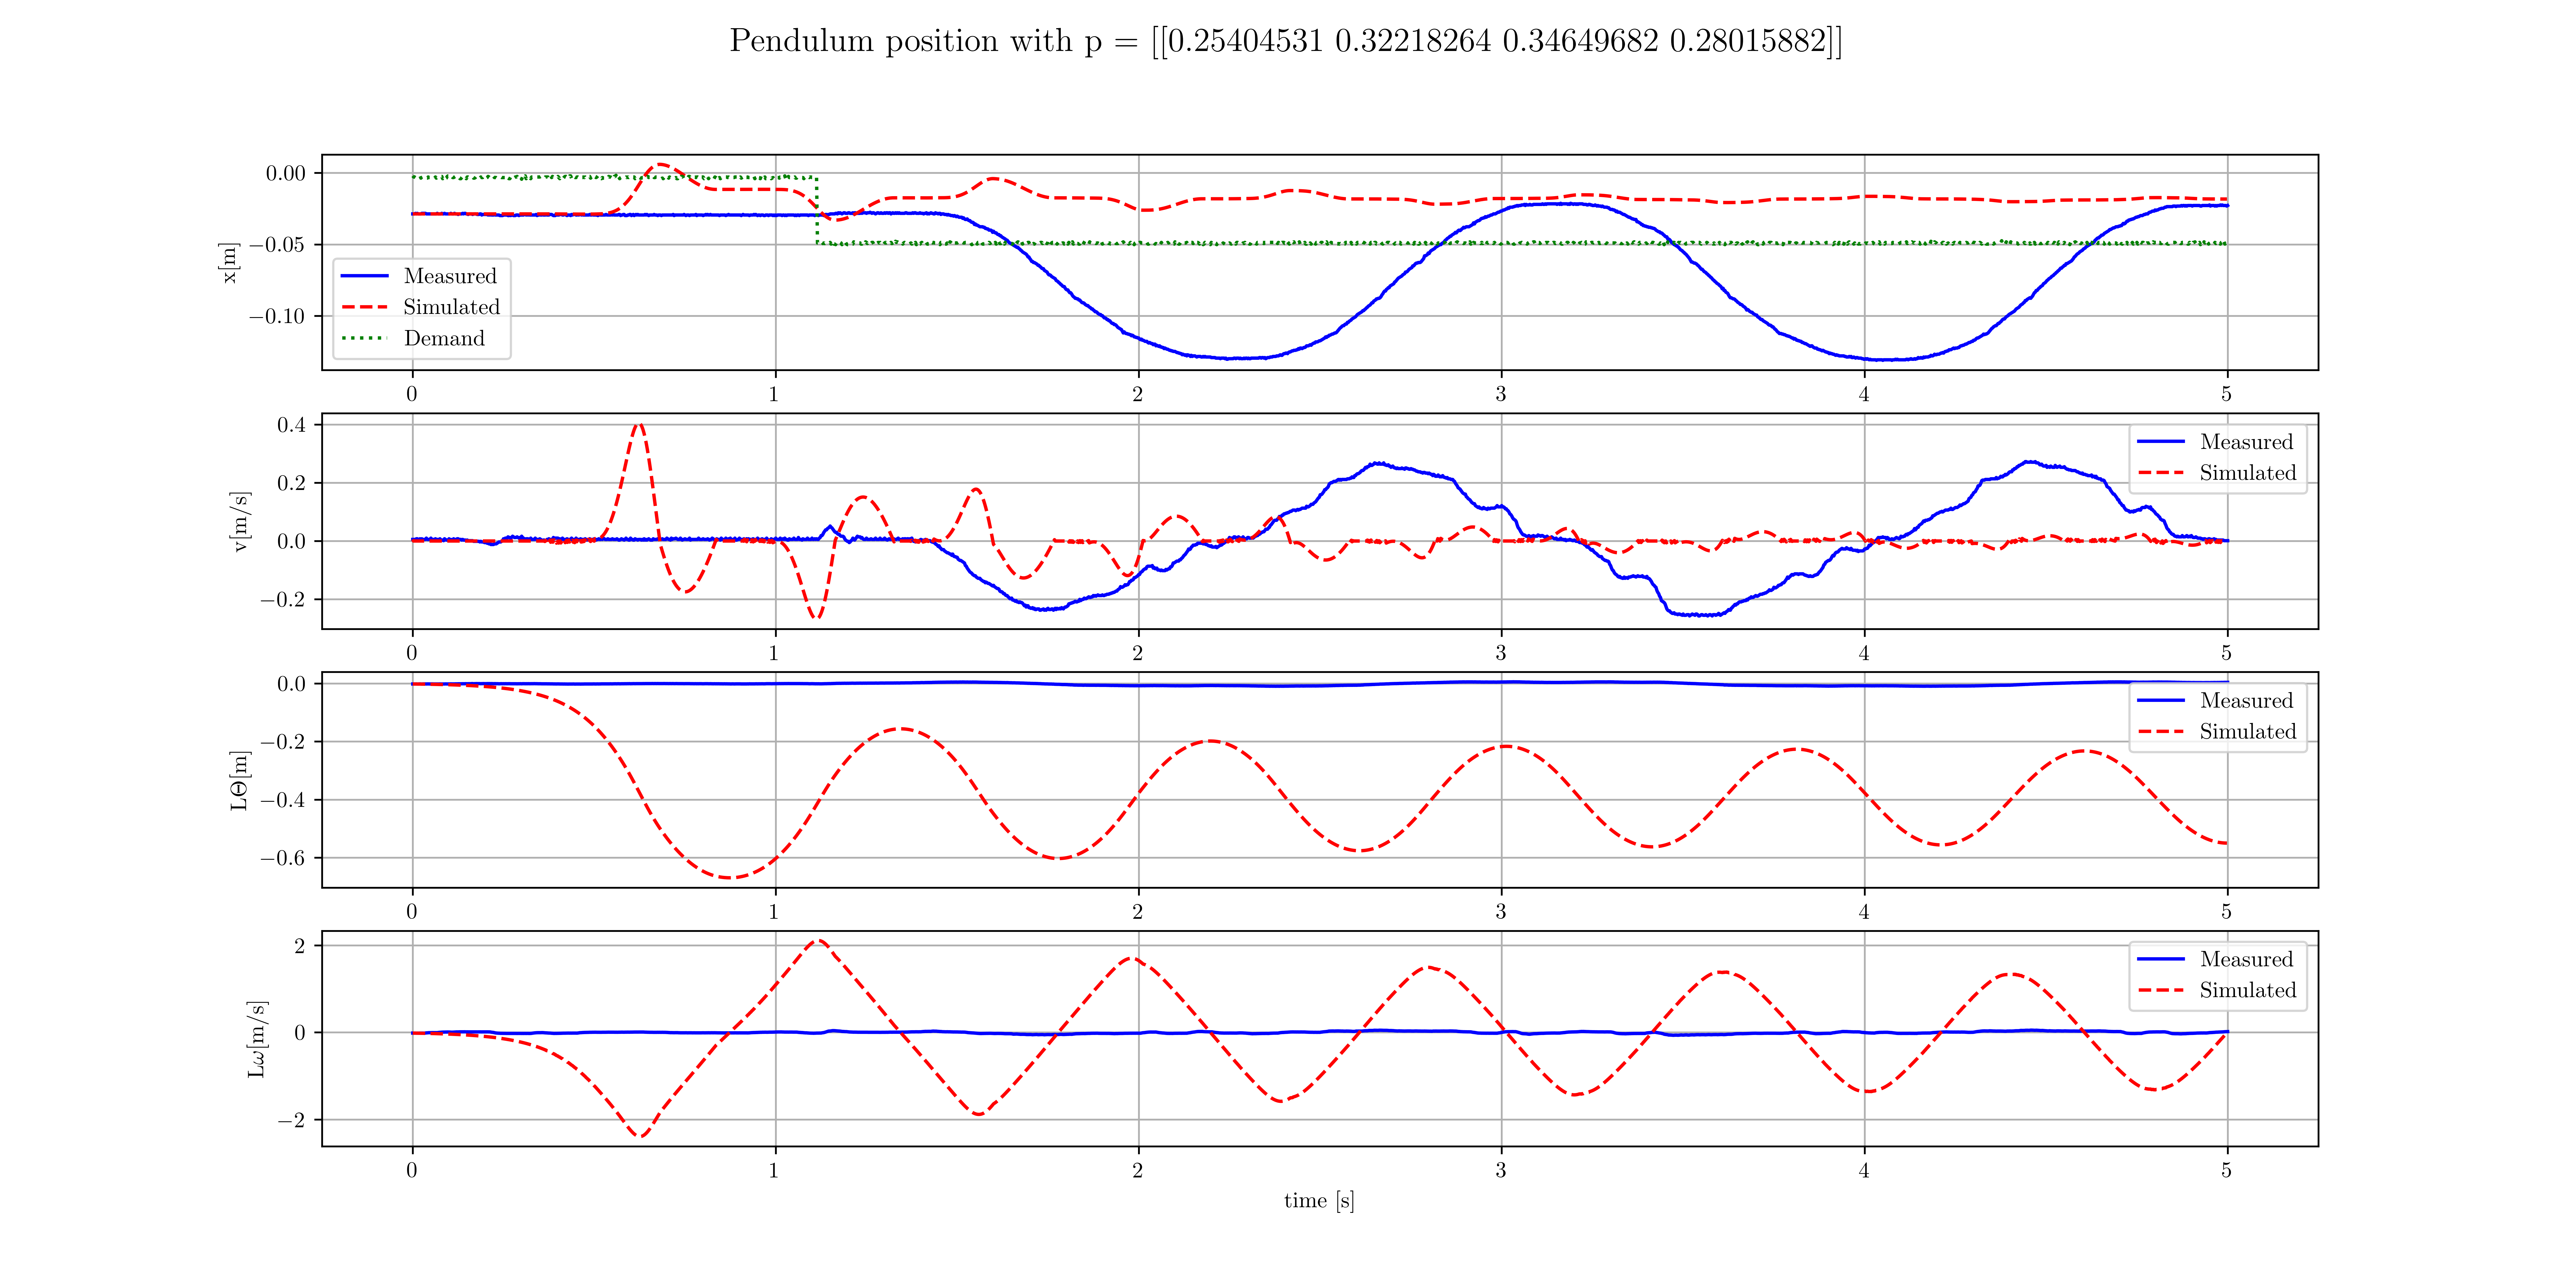
\includegraphics[width=0.99\textwidth]{figures/4.3.png}
  \caption{Inverted pendulum root locus for varying $k_2$ only}
  \label{fig:4.3}
\end{figure}

% 4.4 limit cycles
\subsubsection{Limit Cycles}

\begin{figure}[H]
  \centering
  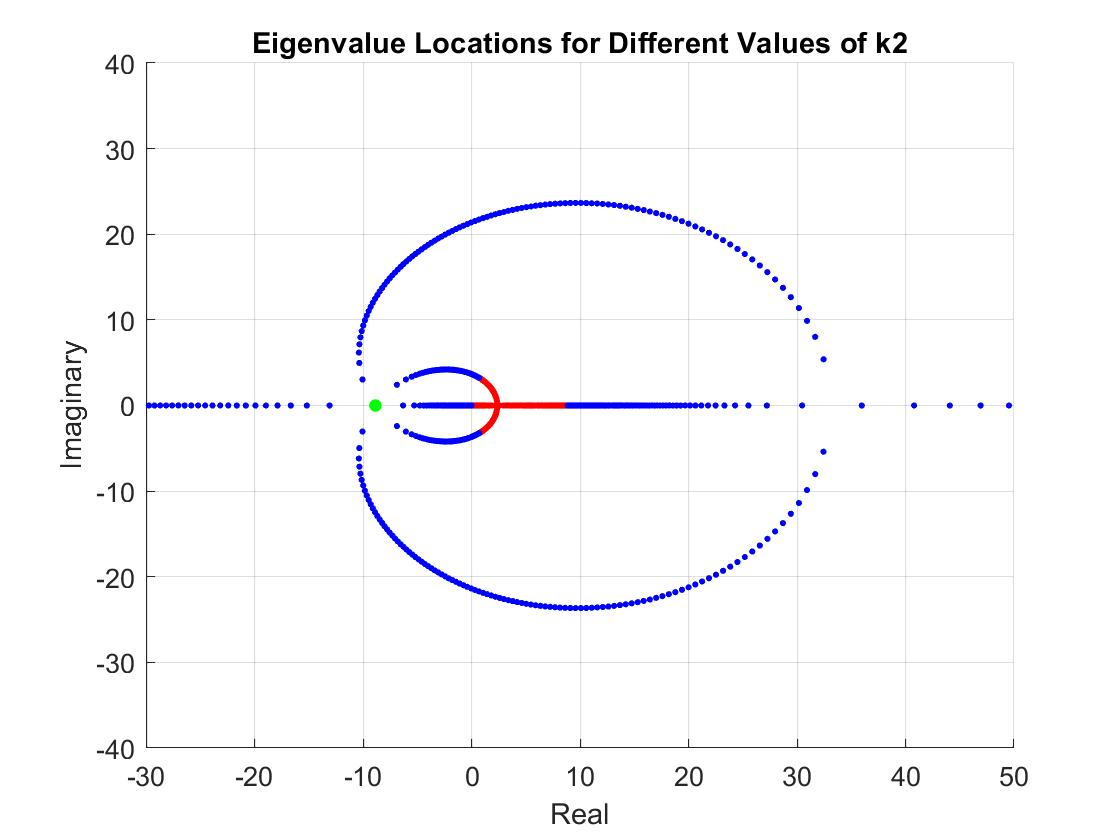
\includegraphics[width=0.7\textwidth]{figures/4.4roots.jpg}
  \caption{Inverted pendulum root locus for varying $k_2$ only}
  \label{fig:roots4.4}
\end{figure}

\begin{figure}[H]
  \centering
  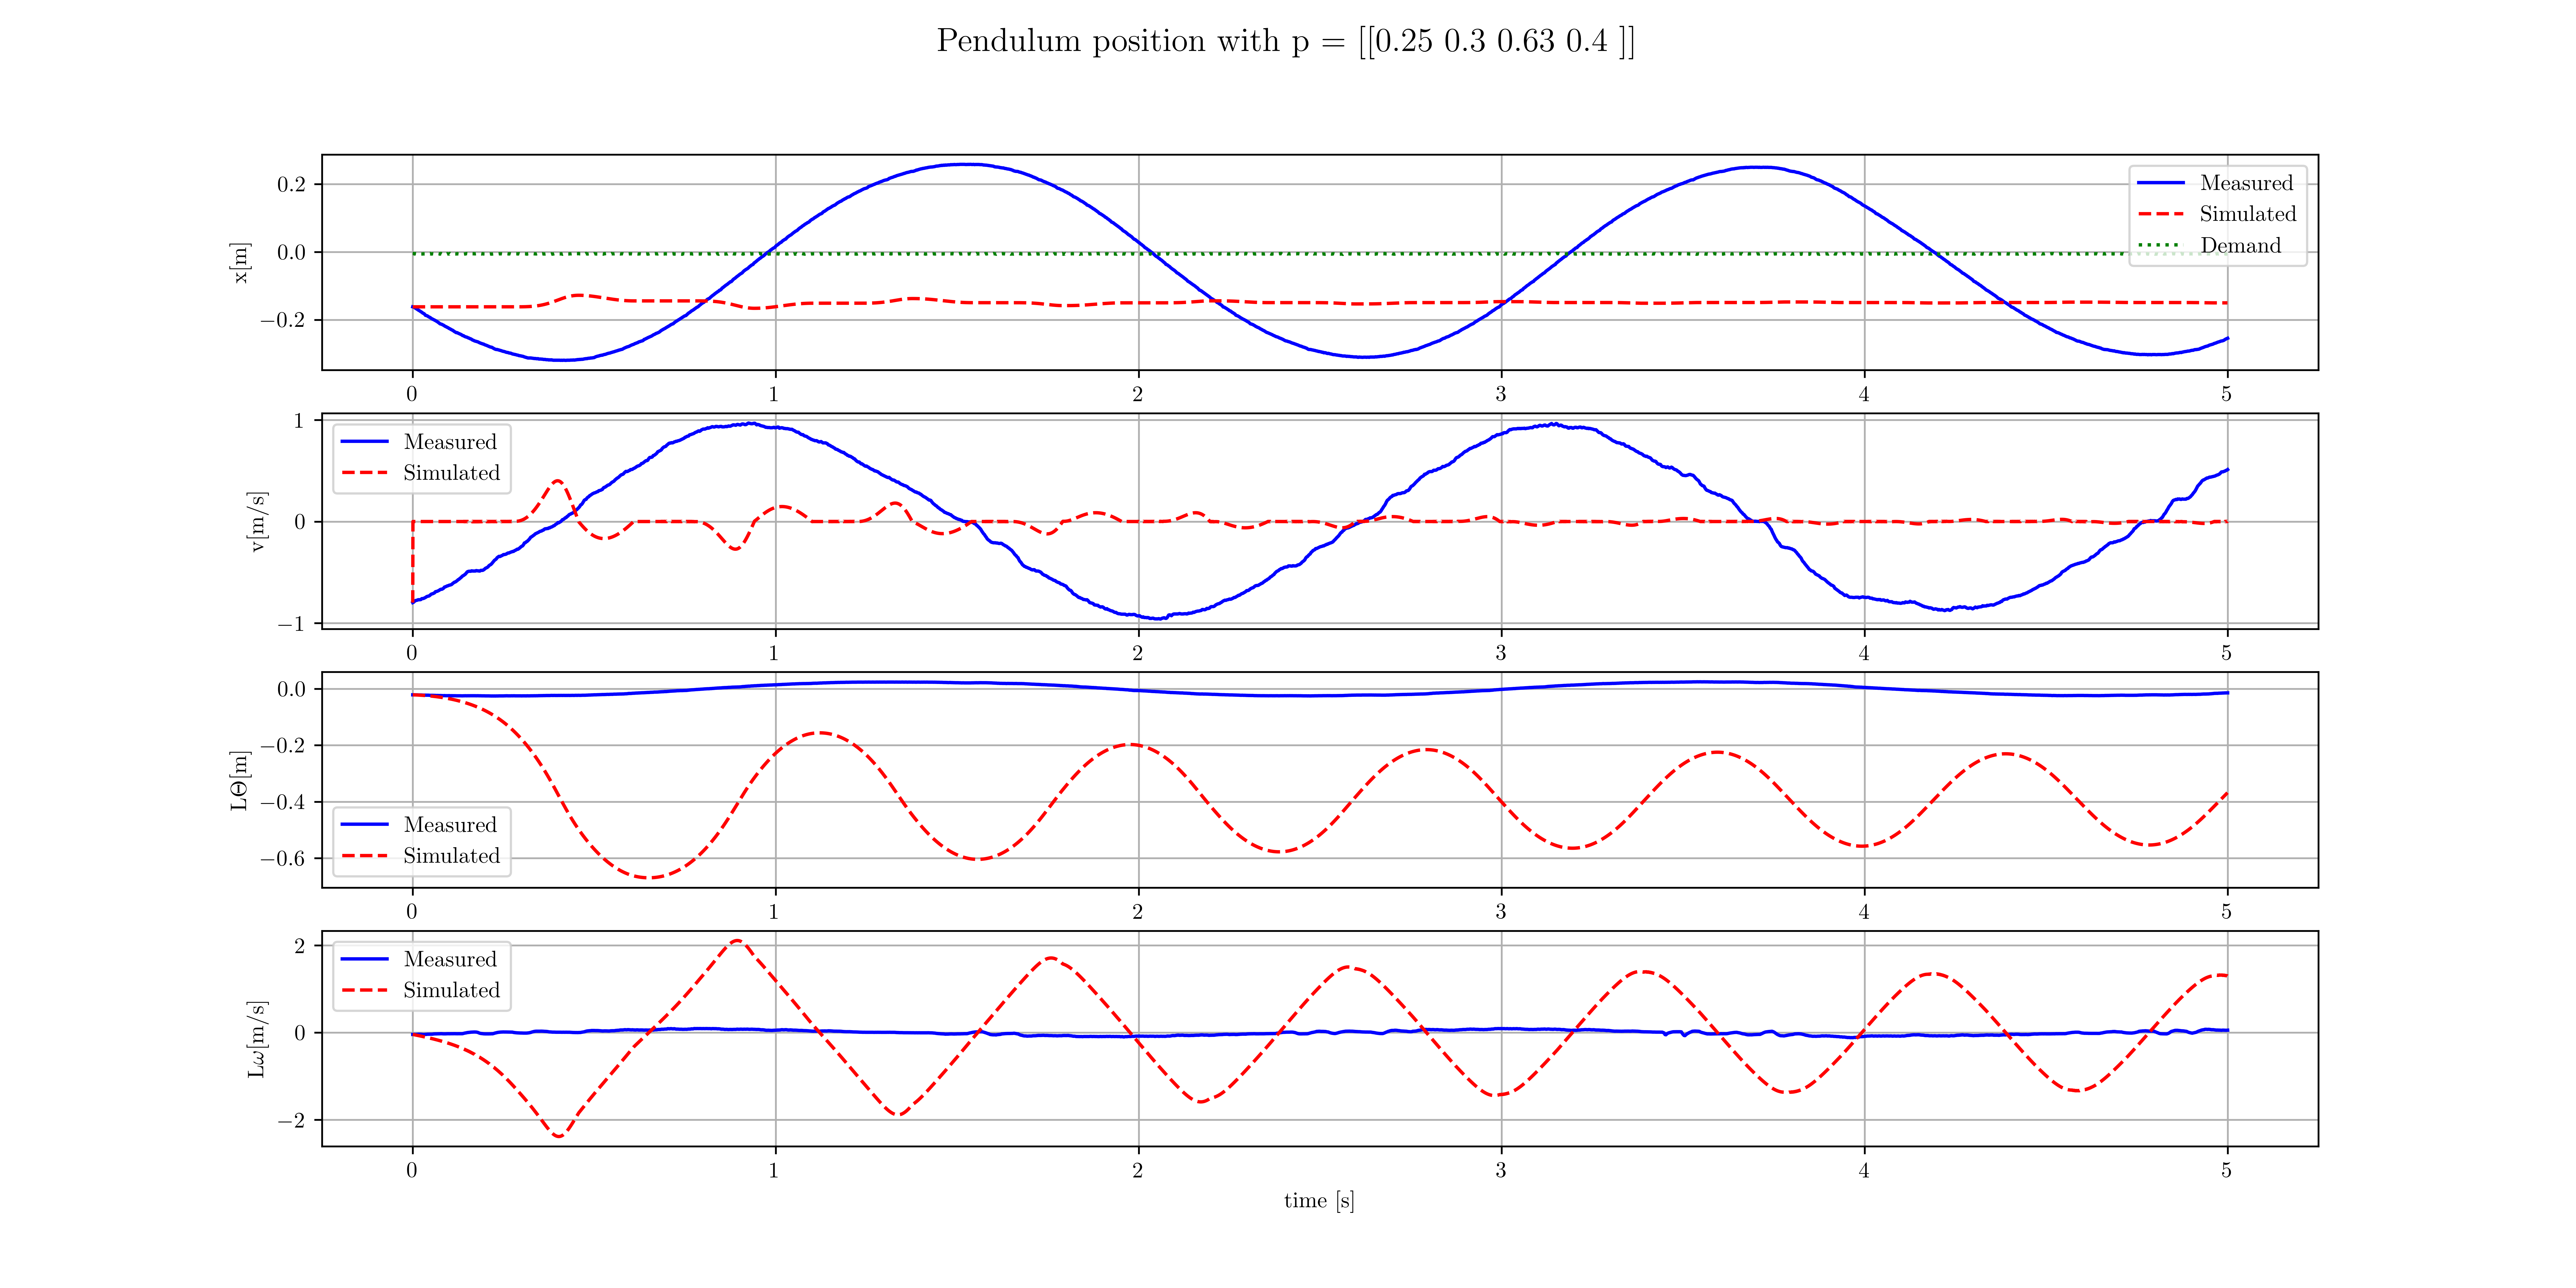
\includegraphics[width=0.99\textwidth]{figures/4.4_lo.png}
  \caption{Inverted pendulum response at minimum $k_2 = $ for stability}
  \label{fig:roots4.4_lo}
\end{figure}

Figure \ref{fig:roots4.4_lo} shows the response at the onset of instability at a lower bound of $p_2 = 0.30$.
Large oscillations were observed 
This can be seen in the poles $-1.27029093 \pm 2.37834982j$
These have a small imaginary component and so have a lower frequency, as observed.
The value of damping is also small which is given by the real part.

\begin{figure}[H]
  \centering
  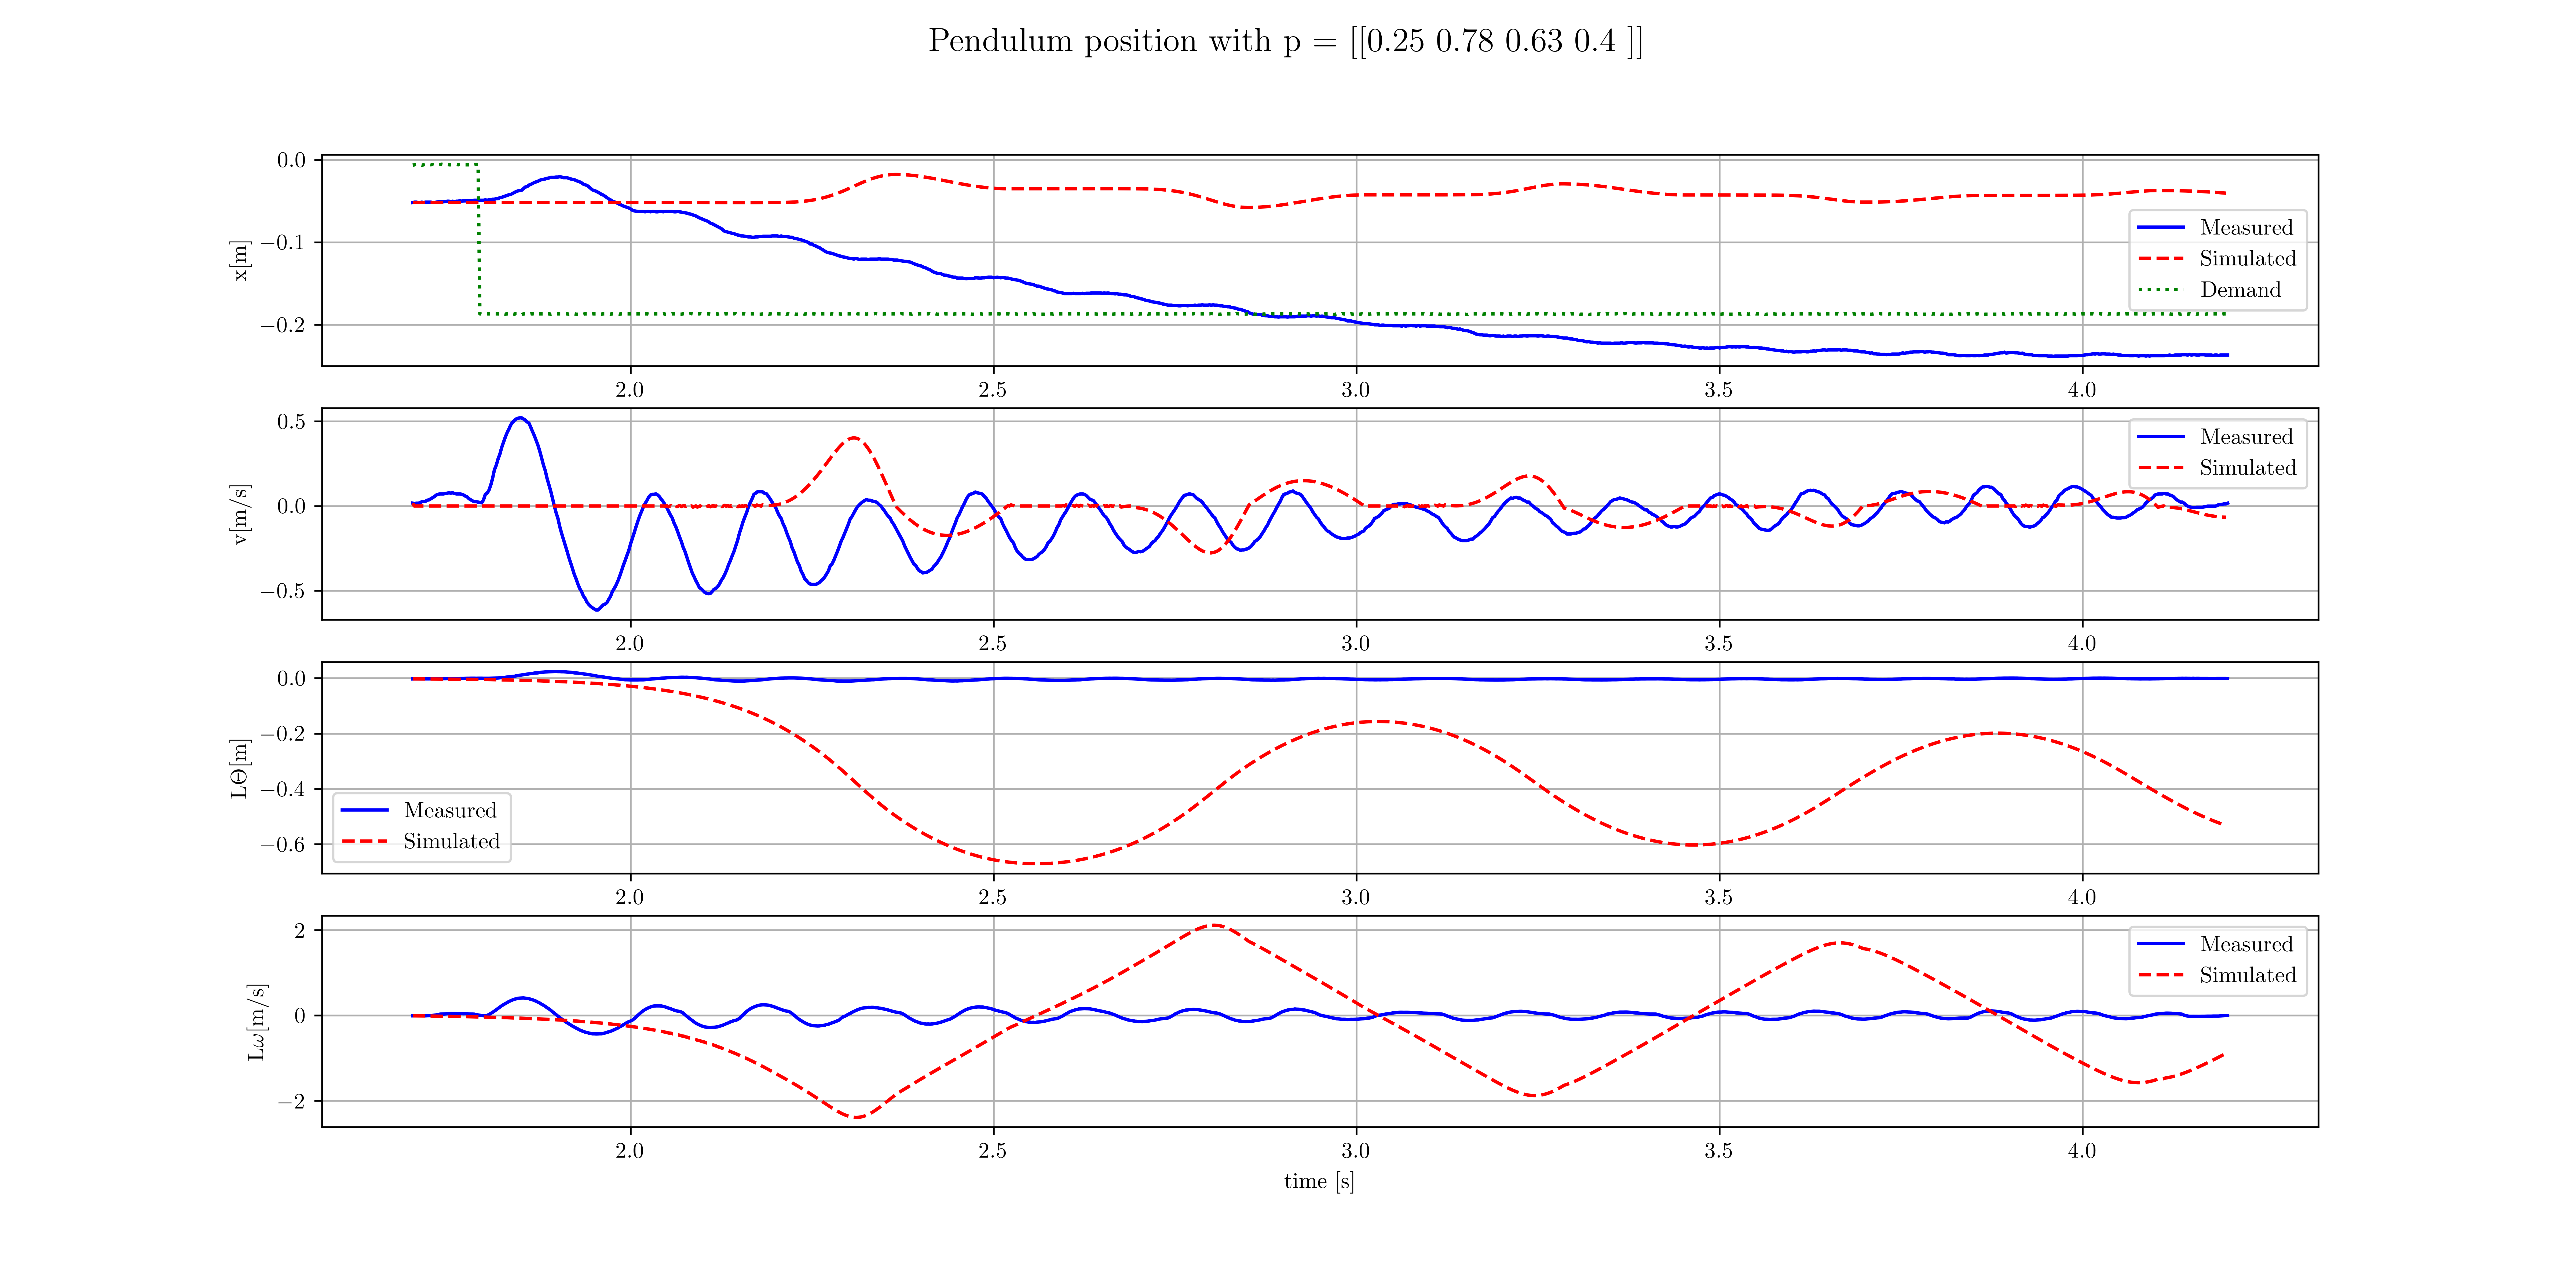
\includegraphics[width=0.99\textwidth]{figures/4.4_hi.png}
  \caption{Inverted pendulum response at maximum $k_2 = $ for stability}
  \label{fig:roots4.4_hi}
\end{figure}

Figure \ref{fig:roots4.4_hi} shows the response at the onset of instability at an upper bound of $p_2 = 0.78$.
The carriage velocity amplitude halves after approximately 7 cycles giving a damping ratio of $\zeta \approx 0.016$
The frequency of carriage velocity is calculated to be about 44 rad/s
This gives the approximated poles of $-0.7 \pm 44j$

The calculated poles of the system are $-4.07147154 \pm 30.42971361j$
This shows that the damping is higher than expected 

\subsubsection{No pendulum feedback}


\subsection{Inverted Pendulum LQR}


%\fi


\section{Conclusion}


\newpage
\section{Appendix}

\subsection{Transfer functions}

\begin{align}
  \left( 1 + \frac{M}{m} + \frac{I}{ma^2} \right) \ddot{x} &= \frac{T}{ma} - \frac{F}{m}\text{sgn}(\dot{x}) - l\sin\phi . \ddot{\phi} - l\cos\phi . \dot{\phi}^2 \\
   - l \ddot{\phi} &= \sin\phi \ddot{x} - g\cos\phi
\end{align}

Crane closed loop transfer function
\begin{equation}
  \mathbf{C} (s\mathbf{I} - \mathbf{A} + \mathbf{KB}) ^{-1} \mathbf{B} = \left[\begin{matrix}\frac{617.283950617284 \left(\omega_{1}^{2} + s^{2}\right)}{k_{1} \omega_{1}^{2} + k_{1} s^{2} + k_{2} \omega_{1}^{2} s + k_{2} s^{3} + k_{3} s^{2} + k_{4} s^{3} + \omega_{0}^{2} s^{2} + s^{4}}\\\frac{165.185185185185 s \left(\omega_{1}^{2} + s^{2}\right)}{k_{1} \omega_{1}^{2} + k_{1} s^{2} + k_{2} \omega_{1}^{2} s + k_{2} s^{3} + k_{3} s^{2} + k_{4} s^{3} + \omega_{0}^{2} s^{2} + s^{4}}\\\frac{1256.2962962963 s^{2}}{k_{1} \omega_{1}^{2} + k_{1} s^{2} + k_{2} \omega_{1}^{2} s + k_{2} s^{3} + k_{3} s^{2} + k_{4} s^{3} + \omega_{0}^{2} s^{2} + s^{4}}\\- \frac{126.41975308642 s^{3}}{k_{1} \omega_{1}^{2} + k_{1} s^{2} + k_{2} \omega_{1}^{2} s + k_{2} s^{3} + k_{3} s^{2} + k_{4} s^{3} + \omega_{0}^{2} s^{2} + s^{4}}\end{matrix}\right]
\end{equation}

Inverted pendulum closed loop transfer function

\begin{equation}
  \mathbf{C} (s\mathbf{I} - \mathbf{A} + \mathbf{KB}) ^{-1} \mathbf{B} = \left[\begin{matrix}\frac{617.283950617284 \left(- \omega_{1}^{2} + s^{2}\right)}{- k_{1} \omega_{1}^{2} + k_{1} s^{2} - k_{2} \omega_{1}^{2} s + k_{2} s^{3} + k_{3} s^{2} + k_{4} s^{3} - \omega_{0}^{2} s^{2} + s^{4}}\\\frac{165.185185185185 s \left(- \omega_{1}^{2} + s^{2}\right)}{- k_{1} \omega_{1}^{2} + k_{1} s^{2} - k_{2} \omega_{1}^{2} s + k_{2} s^{3} + k_{3} s^{2} + k_{4} s^{3} - \omega_{0}^{2} s^{2} + s^{4}}\\\frac{1256.2962962963 s^{2}}{- k_{1} \omega_{1}^{2} + k_{1} s^{2} - k_{2} \omega_{1}^{2} s + k_{2} s^{3} + k_{3} s^{2} + k_{4} s^{3} - \omega_{0}^{2} s^{2} + s^{4}}\\- \frac{126.41975308642 s^{3}}{- k_{1} \omega_{1}^{2} + k_{1} s^{2} - k_{2} \omega_{1}^{2} s + k_{2} s^{3} + k_{3} s^{2} + k_{4} s^{3} - \omega_{0}^{2} s^{2} + s^{4}}\end{matrix}\right]
\end{equation}

% bibliography
\newpage
\begin{thebibliography}{9}

\bibitem{handout}
  G. Vinnicombe,
  \emph{Inverted Pendulum Lab Handout}.
  University of Cambridge,
  2022.

\bibitem{feedback_control_of_dynamic_systems}
  G. F. Franklin, J. D. Powell, A. Emami-Naeini,
  \emph{Feedback Control of Dynamic Systems}.
  Pearson,
  2015.

\bibitem{non_linear_systems}
  H. K. Khalil,
  \emph{Nonlinear Systems}.
  Pearson,
  2002.

\bibitem{modern_control_systems}
  R. C. Dorf, R. H. Bishop,
  \emph{Modern Control Systems}.
  Pearson,
  2016.

\end{thebibliography}

\end{document}